%% ===============================================================================
%%  22AIE437 Medical Image Processing -- Final Project Report
%%  Elsevier CAS single-column template (cas-sc)
%%  Compile: pdflatex report && bibtex report && pdflatex report && pdflatex report
%%           (or upload the report/ folder to Overleaf)
%% ===============================================================================
\documentclass[a4paper,fleqn]{cas-sc}

\usepackage[authoryear]{natbib}
\usepackage{booktabs}
\usepackage{multirow}
\usepackage{amsmath,amssymb}
\usepackage{graphicx}
\usepackage{xcolor}
\graphicspath{{figures/}}
% red placeholders: replace every \fillme{...} with the real group details before submission
\newcommand{\fillme}[1]{\textcolor{red}{\textbf{[#1]}}}
% the class always prints an "ORCID(s):" footnote; we list no ORCIDs, so switch it off
\RenewDocumentCommand{\printorcid}{}{}

\begin{document}
\let\WriteBookmarks\relax
\def\floatpagepagefraction{1}
\def\textpagefraction{.001}

\shorttitle{Improving CAR-UNet for retinal vessel segmentation on FIVES}
\shortauthors{Group \fillme{No.}}

\title [mode = title]{Seeing the thin vessels: replicating and improving Channel Attention Residual U-Net for retinal vessel segmentation on the multi-disease FIVES dataset}

\tnotemark[1]
\tnotetext[1]{Final project report, course 22AIE437 Medical Image Processing, B.Tech CSE (AI), Amrita School of Artificial Intelligence. \textbf{Group \fillme{Group No. / Name}.} Members and roll numbers: Abhishek Karthik J (\fillme{Roll No.}); \fillme{Member 2} (\fillme{Roll No.}); \fillme{Member 3} (\fillme{Roll No.}); \fillme{Member 4} (\fillme{Roll No.}).}

\author[1]{Abhishek Karthik J}
\author[1]{\fillme{Member 2}}
\author[1]{\fillme{Member 3}}
\author[1]{\fillme{Member 4}}

\affiliation[1]{organization={Amrita School of Artificial Intelligence, Amrita Vishwa Vidyapeetham},
    country={India}}

\begin{abstract}
The retina is the only place in the body where blood vessels can be photographed directly and non-invasively, and changes in their calibre, branching and continuity are early signs of diabetic retinopathy, glaucoma and hypertension. Automatic vessel segmentation is therefore a key step in fundus-image screening, but even strong networks still miss the thinnest capillaries. In this work we replicate the Channel Attention Residual U-Net (CAR-UNet) of \citet{guo2021carunet} on FIVES, a public dataset of 800 high-resolution fundus images covering normal eyes, age-related macular degeneration, diabetic retinopathy and glaucoma, using a strict protocol: a disease-stratified split, identical training settings for all models, three training seeds, all 200 test images and paired significance tests. The replicated CAR-UNet reaches a Dice score of $0.8382 \pm 0.0031$ and outperforms a plain U-Net on 154 of 200 test images. We then address four weaknesses of the base model: we add spatial attention to its channel attention (dual attention), train with a topology-aware clDice loss, work at $1024 \times 1024$ instead of $512 \times 512$ pixels, and select the decision threshold on the validation set. The improved model reaches a Dice score of $0.8436 \pm 0.0027$, an IoU of 0.7379 and a centreline Dice (clDice) of 0.8751, improves vessel connectivity on 175 of 200 test images ($p = 5 \times 10^{-25}$) and gains 2.2 Dice points when scored against the full-resolution ground truth. An ablation study shows the contribution of each component, and we report honestly where the approach does not help.
\end{abstract}

\begin{keywords}
Retinal vessel segmentation \sep Fundus images \sep CAR-UNet \sep Attention mechanisms \sep clDice \sep FIVES dataset
\end{keywords}

\maketitle

%% ===============================================================================
\section{Introduction}
\label{sec:intro}

The retina offers a rare, non-invasive view of the body's microvasculature. A single fundus photograph shows arteries, veins and capillaries whose width, tortuosity, branching pattern and continuity change with diabetic retinopathy (DR), glaucoma, age-related macular degeneration (AMD) and hypertension. Measuring these changes requires a vessel map, a pixel-wise segmentation of the vascular tree. Producing such maps by hand is slow and tedious, and different experts disagree, especially on the faint capillaries at the ends of the tree. This is exactly where early pathological changes appear, which makes automatic vessel segmentation an attractive target for medical image analysis.

The task is harder than it first appears. In FIVES, vessels make up only about 7\% of the image (about 10\% of the retinal field of view), so any method is pushed towards predicting background. Illumination varies strongly across the image, the optic disc and lesions such as exudates and haemorrhages produce high-contrast structures that resemble vessels, and the thinnest capillaries are only one or two pixels wide once the image is resized to a manageable resolution. Classical approaches based on vesselness filters \citep{frangi1998} handle the large vessels but break down on these thin, low-contrast structures. Deep convolutional networks have largely replaced them \citep{liskowski2016}, with the U-Net encoder--decoder architecture \citep{ronneberger2015unet} becoming the standard backbone. Many variants add attention, among them Attention U-Net \citep{oktay2018attention}, SA-UNet \citep{guo2021saunet} and CAR-UNet \citep{guo2021carunet}, the base paper of this project. CAR-UNet replaces the convolution blocks of U-Net with residual blocks that contain an efficient channel-attention module, and applies the same attention to the skip connections.

CAR-UNet was evaluated on small, single-source benchmarks with 20 to 40 images, such as DRIVE \citep{staal2004drive}, and only with accuracy, sensitivity, specificity and AUC. It is therefore unclear how it behaves on larger, multi-disease data, and whether its design really recovers the thin vessels that matter clinically. Our own replication shows that most of its remaining errors are exactly there: thin capillaries that are missed or broken into pieces.

This report makes the following contributions:
\begin{itemize}
\item We replicate CAR-UNet on FIVES \citep{jin2022fives}, an 800-image dataset with four disease groups, under a strict and reproducible protocol, and compare it with U-Net.
\item We identify five weaknesses of the base model and its evaluation, and propose four targeted modifications: dual (channel + spatial) attention, a topology-aware clDice loss, a higher working resolution, and a validation-selected decision threshold.
\item We evaluate every model with three training seeds on all 200 test images, report Dice, IoU, clDice and the paper's metrics, test every difference with paired Wilcoxon tests, and quantify the contribution of each modification in an ablation study.
\item We analyse the results per disease and on thin vessels, and report the cases where our approach does not help.
\end{itemize}

The rest of the report is organised as follows. Section~\ref{sec:related} reviews related work, Section~\ref{sec:base} describes the base paper and our replication, Section~\ref{sec:method} presents the methodology and the proposed modifications, Section~\ref{sec:results} reports the results, Section~\ref{sec:discussion} discusses them, and Section~\ref{sec:conclusion} concludes.

%% ===============================================================================
\section{Related work}
\label{sec:related}

\paragraph{Vessel segmentation.} Early methods enhanced tubular structures with Hessian-based filters \citep{frangi1998} or matched filters and then thresholded the response. Supervised deep networks now dominate. \citet{liskowski2016} showed that convolutional networks trained on image patches clearly outperform hand-crafted pipelines, and the U-Net \citep{ronneberger2015unet}, with its contracting path, expanding path and skip connections, has become the most common backbone because it combines context with precise localisation.

\paragraph{Attention and residual learning.} Residual connections \citep{he2016resnet} make deeper networks easier to optimise. Channel attention, introduced with squeeze-and-excitation networks \citep{hu2018se} and made lightweight by ECA-Net \citep{wang2020eca}, reweights feature channels. CBAM \citep{woo2018cbam} combines channel attention with spatial attention that reweights image locations. In retinal imaging, Attention U-Net \citep{oktay2018attention} gates the skip connections, SA-UNet \citep{guo2021saunet} uses spatial attention, and CAR-UNet \citep{guo2021carunet} builds residual blocks around a modified efficient channel attention (MECA).

\paragraph{Losses and topology.} Cross-entropy and the soft Dice loss \citep{milletari2016vnet} are the usual training objectives, but both count pixels and are almost blind to whether a thin vessel is connected. The clDice loss \citep{shit2021cldice} compares the skeletons of prediction and ground truth and was designed for tubular structures such as vessels.

\paragraph{Datasets.} DRIVE \citep{staal2004drive} and similar benchmarks contain a few dozen images from a single source. FIVES \citep{jin2022fives} provides 800 images at $2048 \times 2048$ pixels, with expert-consensus annotations and a balanced mix of normal, AMD, DR and glaucoma cases, which makes it a much more demanding testbed.

%% ===============================================================================
\section{Base paper and replication}
\label{sec:base}

\subsection{The CAR-UNet architecture}

CAR-UNet \citep{guo2021carunet} keeps the U-shaped layout of U-Net (Fig.~\ref{fig:arch_base}). Each encoder and decoder stage, and the bottleneck, is a \emph{channel attention double residual block} (CADRB): two $3\times3$ convolutions with batch normalisation, followed by channel attention, plus a shortcut connection that adds the block input to its output. The channel attention (MECA) pools every feature channel to one number, passes the resulting vector through a small 1D convolution across neighbouring channels and a sigmoid, and multiplies each channel by its weight:
\begin{equation}
\mathbf{F}' = \sigma\!\left(\mathrm{C1D}_k\big(\mathrm{GAP}(\mathbf{F})\big)\right) \odot \mathbf{F},
\label{eq:meca}
\end{equation}
where $\mathrm{GAP}$ is global average pooling, $\mathrm{C1D}_k$ a 1D convolution with kernel size $k$ and $\sigma$ the sigmoid. The same attention is applied to the encoder features on every skip connection before they are concatenated with the decoder features. The paper trains with binary cross-entropy and Adam and reports the results in Table~\ref{tab:paper}; it does not report Dice or IoU.

\begin{figure}[t]
\centering
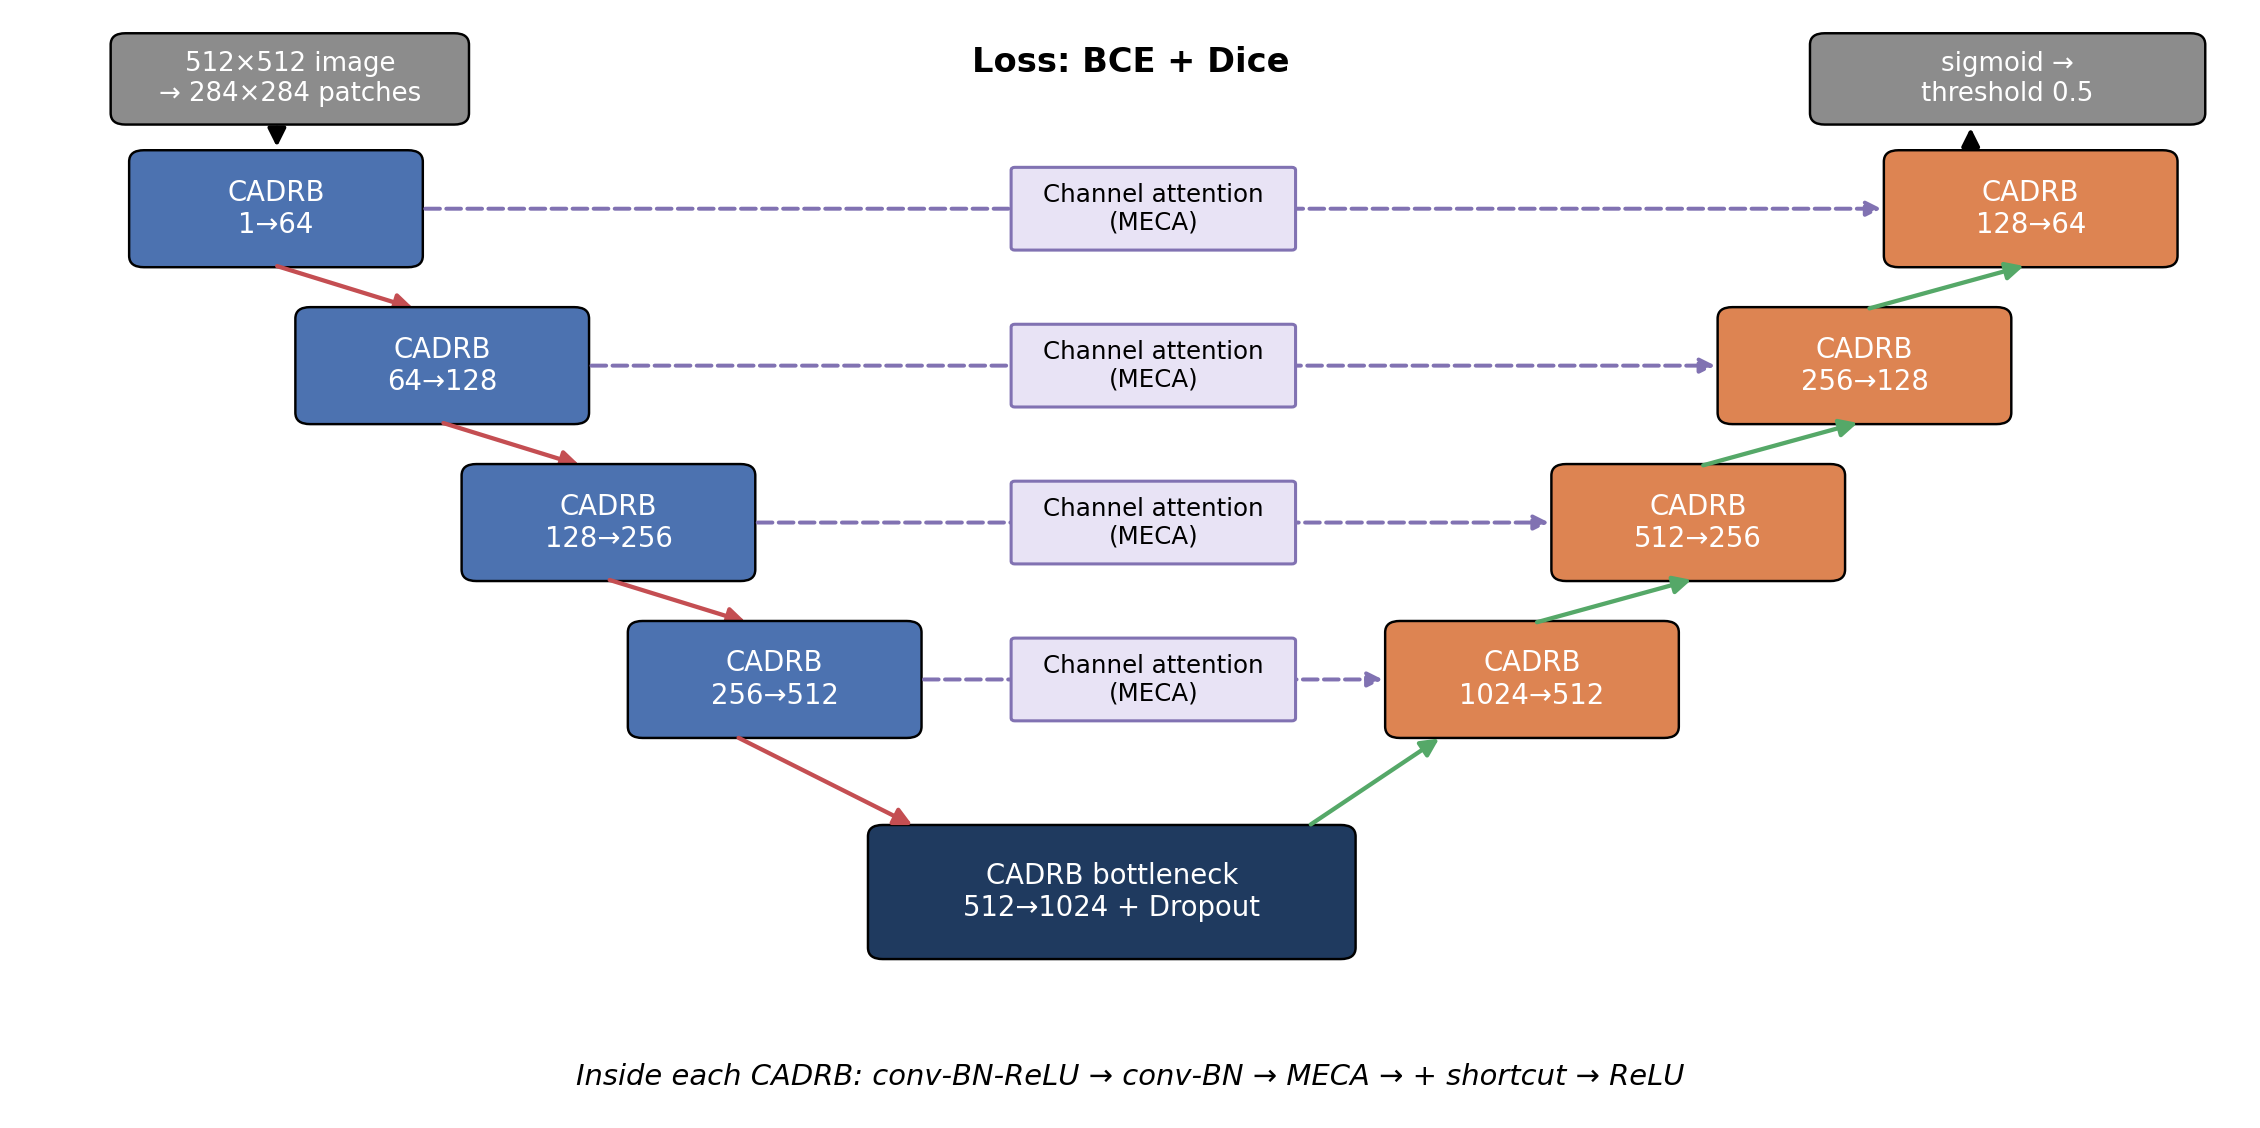
\includegraphics[width=0.92\linewidth]{arch_baseline.png}
\caption{CAR-UNet as implemented in this work. A $284\times284$ input patch is mapped to a $100\times100$ vessel probability map with valid convolutions. Blue: encoder blocks; orange: decoder blocks; dashed arrows: skip connections with channel attention (MECA).}
\label{fig:arch_base}
\end{figure}

\begin{table}[t]
\caption{Results reported in the base paper \citep{guo2021carunet}.}
\label{tab:paper}
\centering
\begin{tabular}{lcccc}
\toprule
Dataset & Accuracy & Sensitivity & Specificity & AUC \\
\midrule
DRIVE & 0.9699 & 0.8135 & 0.9849 & 0.9852 \\
CHASE\_DB1 & 0.9751 & 0.8439 & 0.9839 & 0.9898 \\
STARE & 0.9743 & 0.8445 & 0.9850 & 0.9911 \\
\bottomrule
\end{tabular}
\end{table}

\subsection{Our implementation and its differences from the paper}

We implemented CAR-UNet in PyTorch. To stay consistent with our earlier U-Net baseline we kept the U-Net design with valid convolutions ($284\times284$ input, $100\times100$ output), 64 base filters and dropout in the bottleneck. The original paper uses 16 base filters, DropBlock \citep{ghiasi2018dropblock} and a plain binary cross-entropy loss, and its MECA pools each channel by both average and maximum. We train with a combined cross-entropy and Dice loss (Section~\ref{sec:training}). Our replicated model uses average pooling only, as in Eq.~\eqref{eq:meca}, with an adaptive kernel size $k = |(\log_2 C + 1)/2|_{\text{odd}}$ (minimum 3). The replicated model has 32.4\,M parameters, against 31.0\,M for our U-Net. We state these differences explicitly because they affect absolute numbers.

\subsection{Replication protocol}

A first version of our experiment produced results that turned out to be unreliable, for three main reasons. Only 50 of the 200 test images were scored, and because the filenames were sorted as text, 45 of these 50 were glaucoma images. The validation set contained no DR or glaucoma images. The two models were trained with different settings. We fixed all of these before running any of the experiments reported here. Both models are trained by one script with identical settings (Section~\ref{sec:training}), the validation set is stratified by disease, every model is trained with three seeds, and all 200 test images are scored.

\subsection{Replicated results}

Table~\ref{tab:replication} compares the published results with our replication. A one-to-one comparison is not possible because the datasets differ: the paper used small single-source sets, whereas we use the 800-image multi-disease FIVES dataset. Still, our accuracy, specificity and AUC fall in the same range as the published values, and our sensitivity lies between the paper's DRIVE and CHASE\_DB1 results. More importantly, the replication reproduces the paper's main claim: CAR-UNet is better than U-Net, with a higher Dice on 154 of the 200 test images (paired Wilcoxon test, $p = 2.3\times10^{-14}$). The margin is small (+0.38 Dice points) and varies between seeds (+1.06, $-0.07$ and +0.14 points). Fig.~\ref{fig:samples} shows typical predictions. Thick vessels are traced almost perfectly, while most errors are thin capillaries that are missed or fragmented.

\begin{table}[t]
\caption{Reported versus replicated results. Our results: 200 FIVES test images, mean $\pm$ standard deviation over three training seeds. n/r: not reported.}
\label{tab:replication}
\centering
\small
\setlength{\tabcolsep}{4.5pt}
\begin{tabular}{llcccccc}
\toprule
Model & Dataset & Dice & IoU & Accuracy & Sensitivity & Specificity & AUC \\
\midrule
CAR-UNet (paper) & DRIVE & n/r & n/r & 0.9699 & 0.8135 & 0.9849 & 0.9852 \\
CAR-UNet (paper) & CHASE\_DB1 & n/r & n/r & 0.9751 & 0.8439 & 0.9839 & 0.9898 \\
\midrule
CAR-UNet (ours) & FIVES & $0.8382 \pm 0.0031$ & $0.7295 \pm 0.0043$ & 0.9728 & 0.8310 & 0.9855 & 0.9860 \\
U-Net (ours) & FIVES & $0.8344 \pm 0.0034$ & $0.7246 \pm 0.0050$ & 0.9723 & 0.8247 & 0.9852 & 0.9847 \\
\bottomrule
\end{tabular}
\end{table}

\begin{figure}[t]
\centering
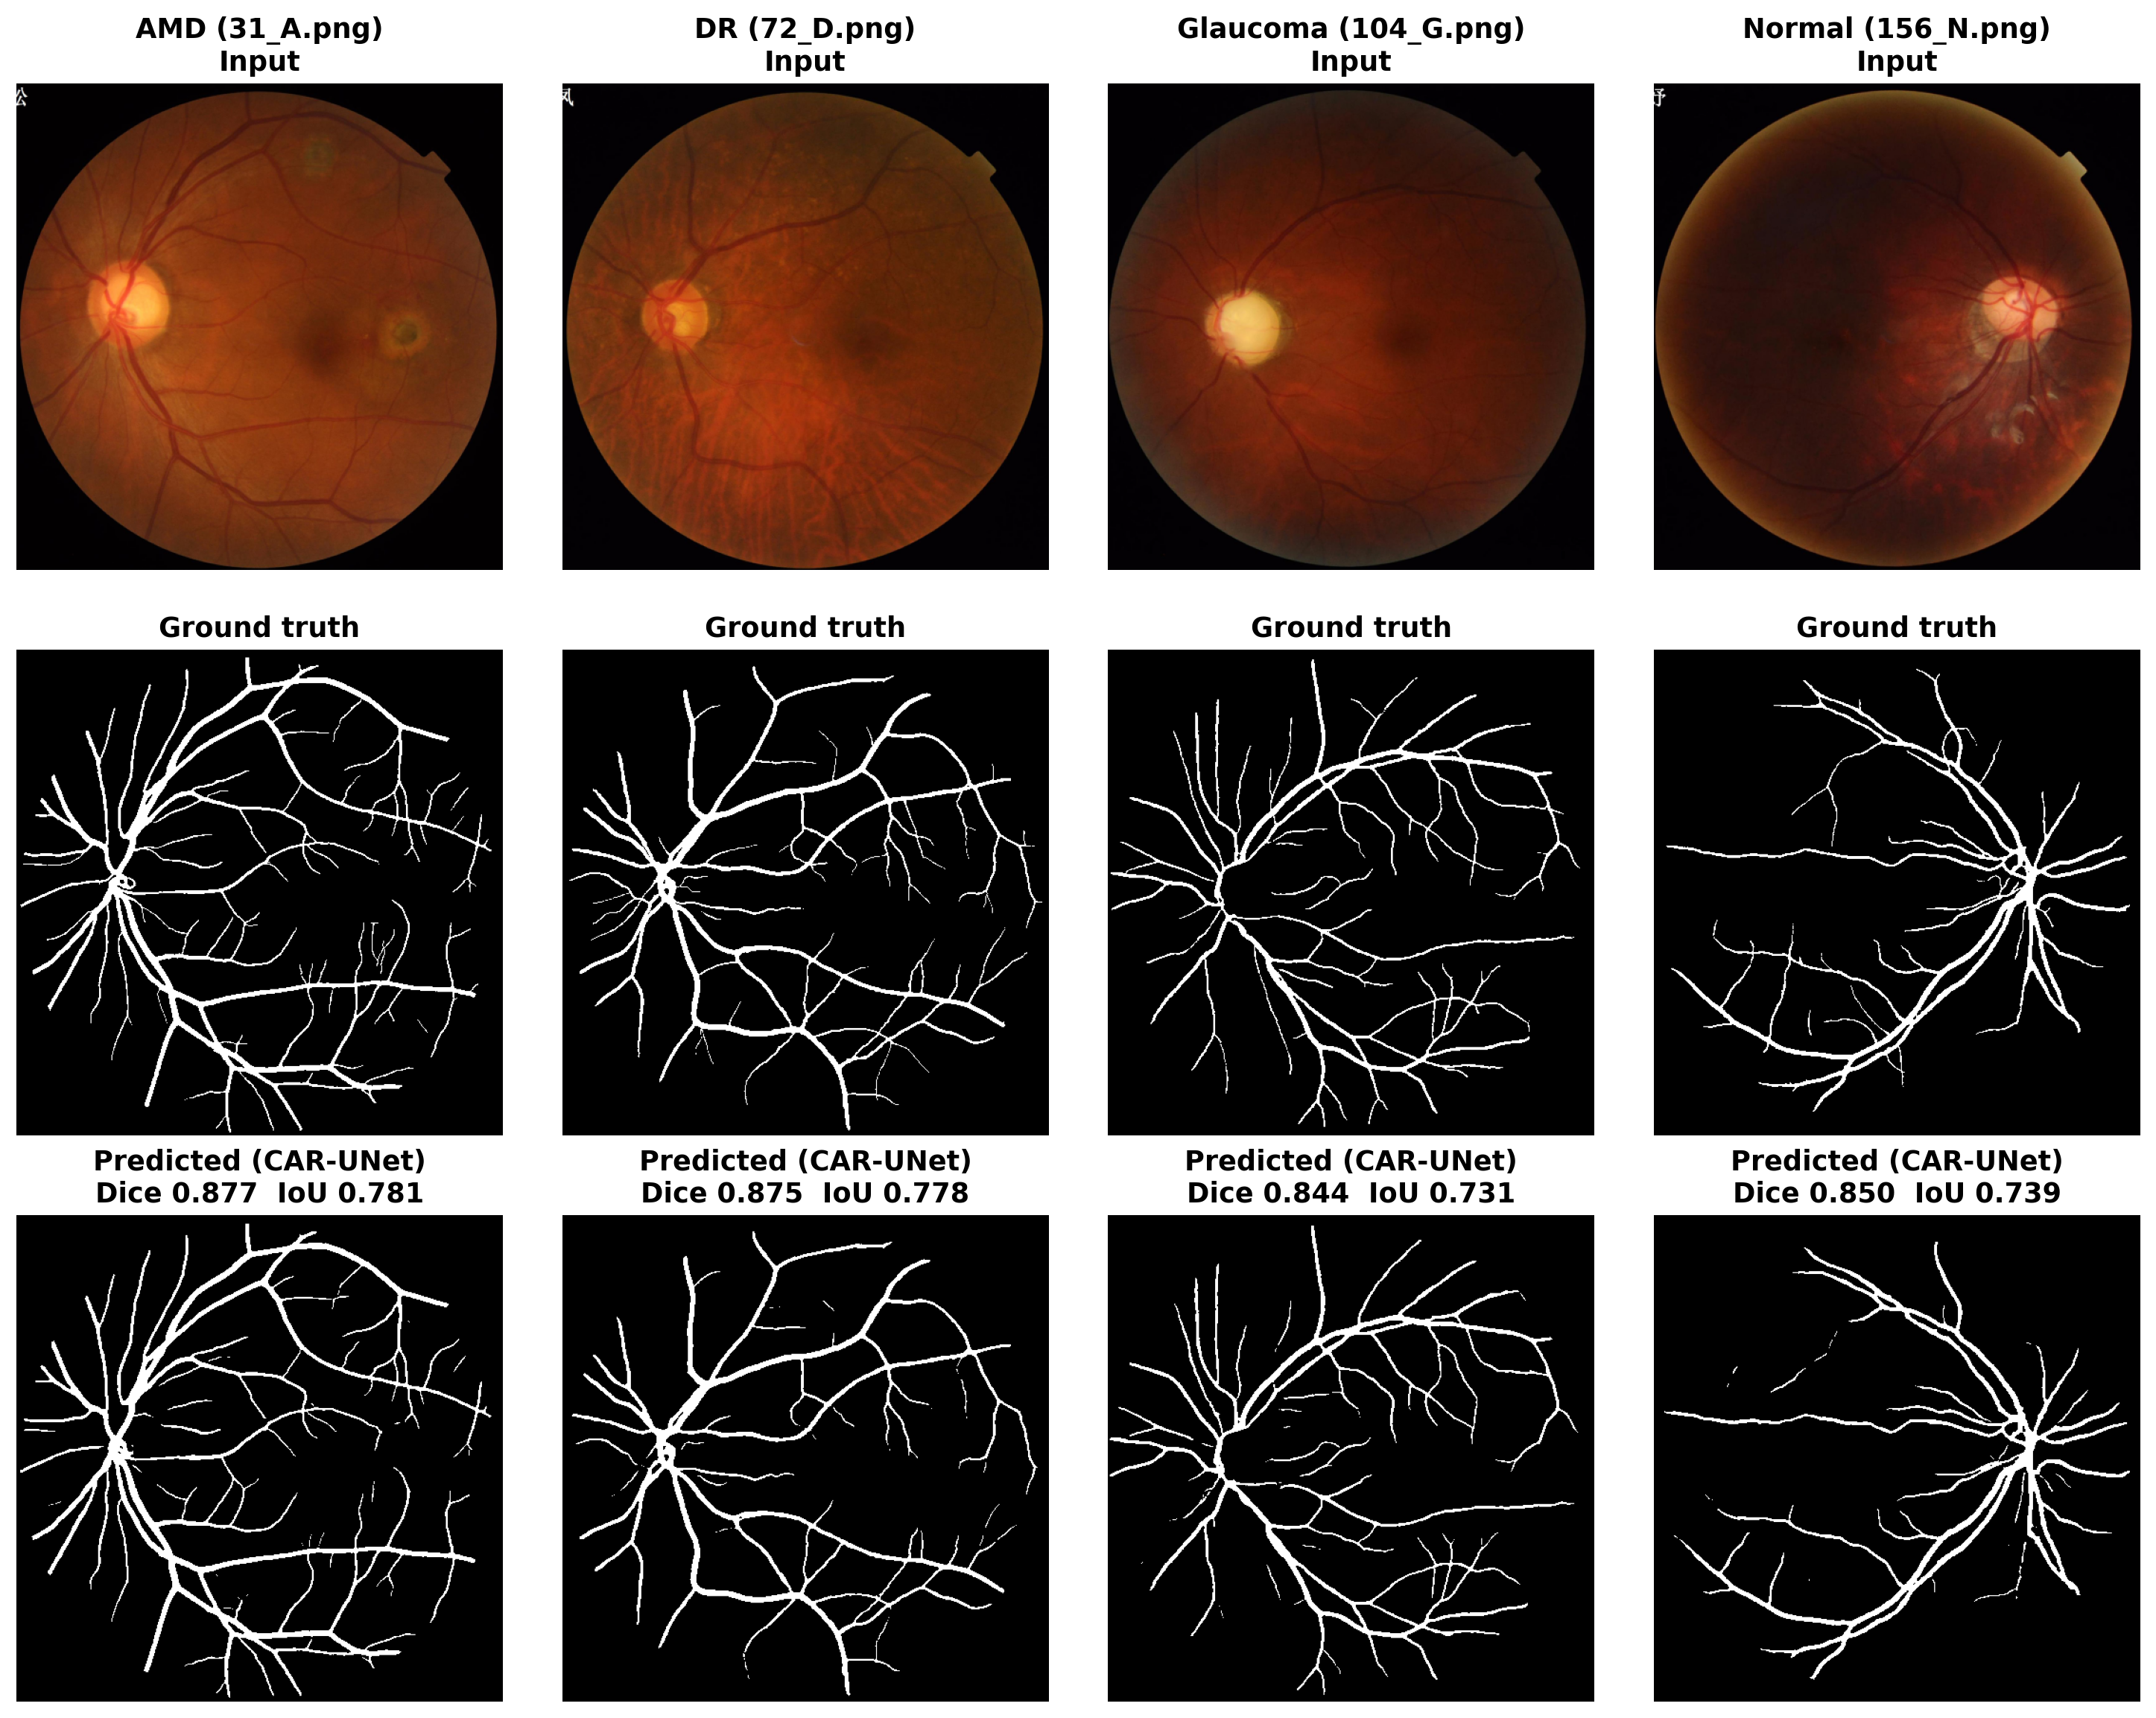
\includegraphics[width=0.80\linewidth]{replicated_samples_all.png}
\caption{Predictions of the replicated CAR-UNet (seed 0) on one test image per disease group, chosen automatically as the image with the median Dice of its group. Rows: input fundus image, expert ground truth, predicted vessel mask with its Dice and IoU.}
\label{fig:samples}
\end{figure}

%% ===============================================================================
\section{Methodology}
\label{sec:method}

Fig.~\ref{fig:pipeline} summarises the full pipeline, from the raw fundus images to the evaluated vessel maps.

\begin{figure}[t]
\centering
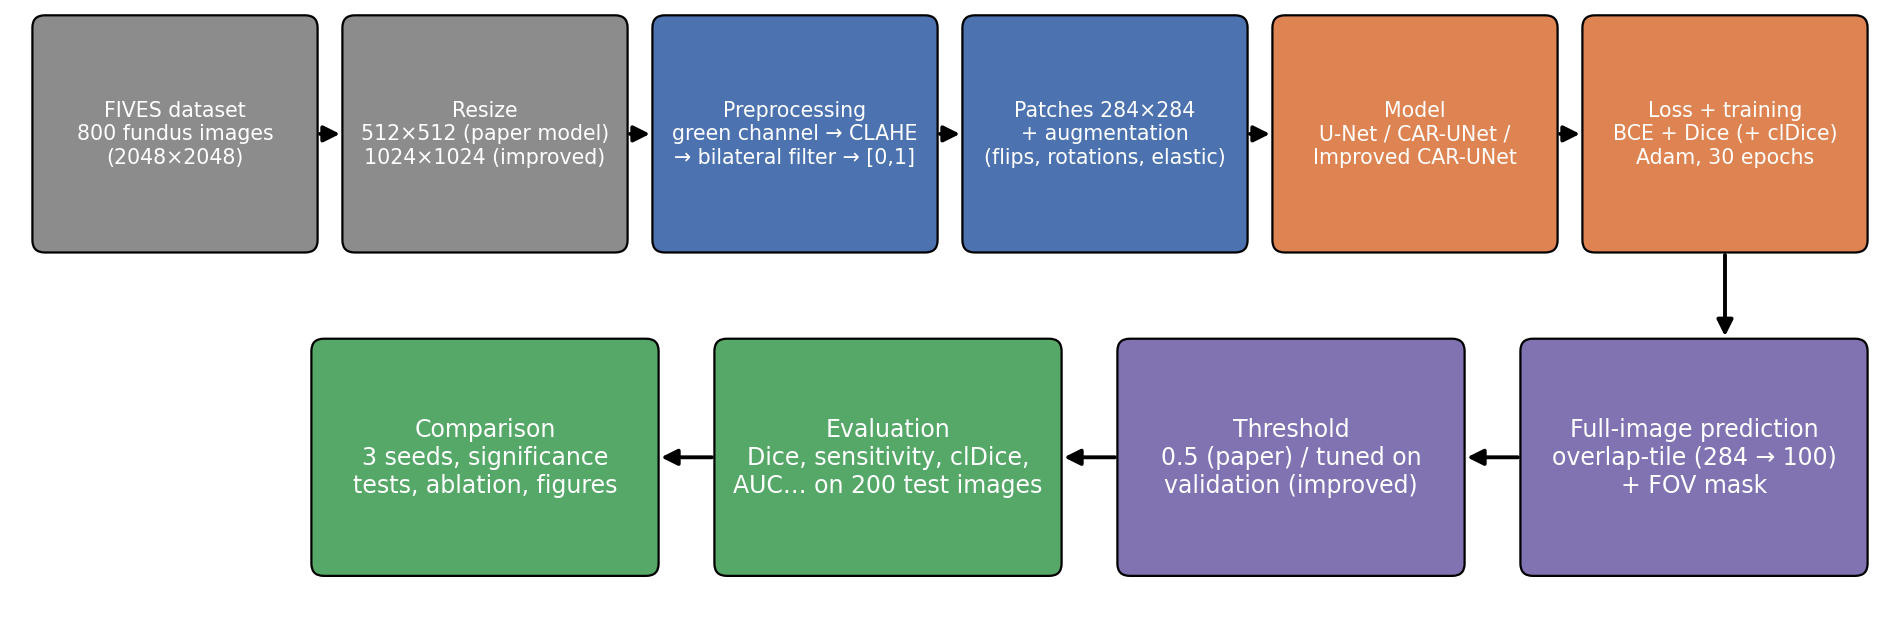
\includegraphics[width=\linewidth]{pipeline.png}
\caption{Overview of the pipeline used for all models.}
\label{fig:pipeline}
\end{figure}

\subsection{Dataset and split}

FIVES \citep{jin2022fives} contains 800 colour fundus images of $2048\times2048$ pixels from 573 patients, annotated by a consensus of ophthalmologists and trained medical staff, with 200 images each of normal eyes, AMD, DR and glaucoma. It comes with an official split into 600 training and 200 test images (50 per group). We divide the 600 training images into 480 for training and 120 for validation, stratified by disease (30 validation images per group) with a fixed seed. The split is made per image, so that no patch of a validation image is ever seen during training. The test set is used only once, for the final evaluation; every choice (best epoch, threshold) is made on the validation set. Images are resized to $512\times512$ for the baseline models and to $1024\times1024$ for the high-resolution model, using area interpolation for images and nearest-neighbour interpolation for masks, so that the masks stay binary.

\subsection{Preprocessing}

Every image goes through the same classical pipeline (Fig.~\ref{fig:preproc}). We keep the green channel, where haemoglobin absorbs most strongly and vessels have the highest contrast. Contrast-limited adaptive histogram equalisation (CLAHE) \citep{zuiderveld1994clahe} (clip limit 2.0, $8\times8$ tiles) compensates for uneven illumination, and an edge-preserving bilateral filter \citep{tomasi1998bilateral} ($d = 5$, $\sigma = 75$) removes noise without blurring the vessel edges. Intensities are then scaled to $[0,1]$. A field-of-view (FOV) mask of the circular retina is computed by thresholding and morphological filtering; all metrics are computed inside it.

\begin{figure}[t]
\centering
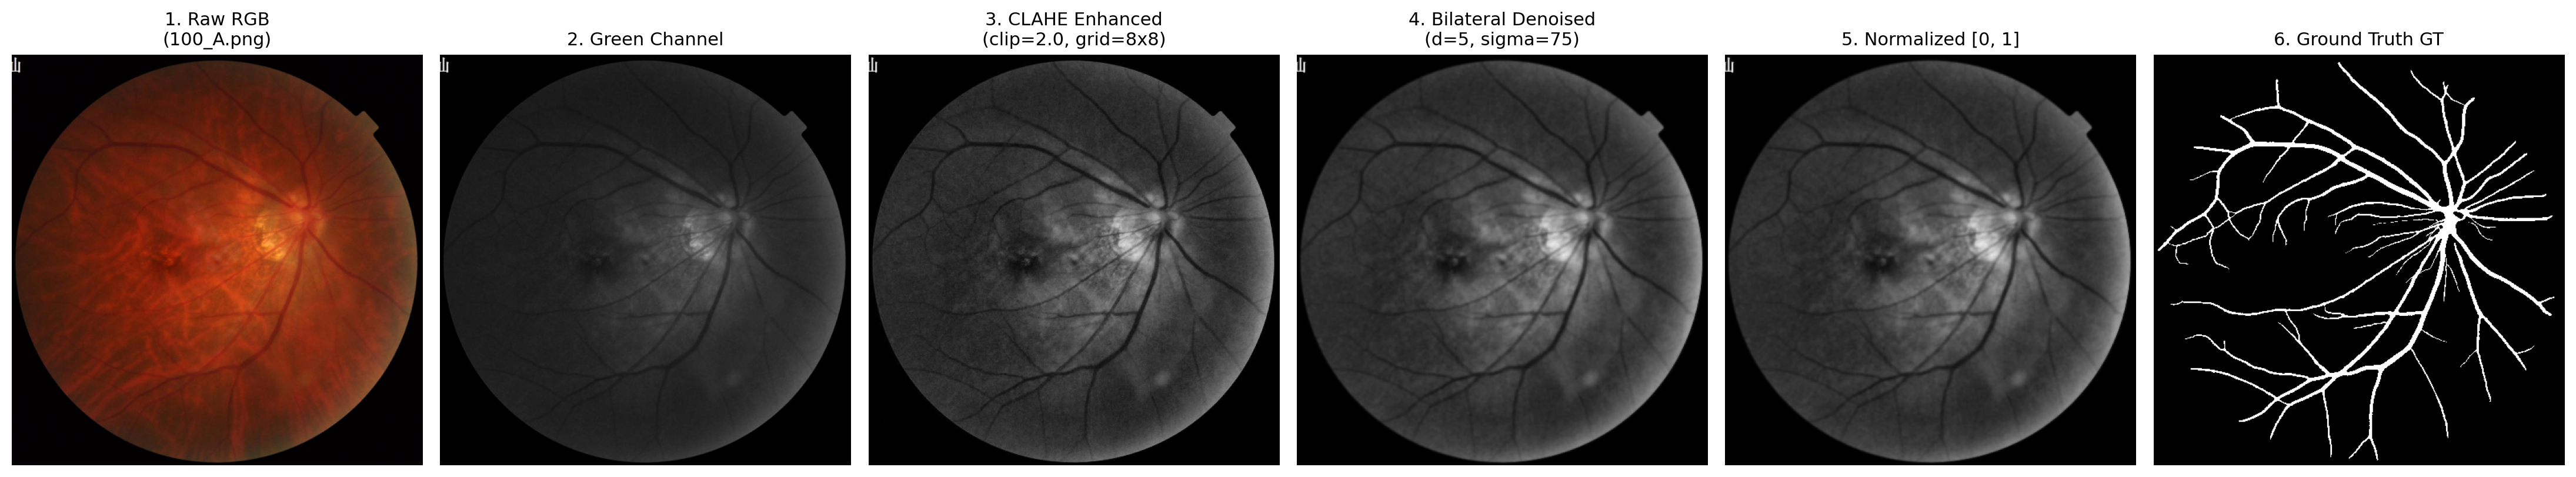
\includegraphics[width=\linewidth]{preprocessing.png}
\caption{Preprocessing of a FIVES training image: RGB input, green channel, CLAHE, bilateral filter, normalised image and the expert ground truth.}
\label{fig:preproc}
\end{figure}

\subsection{Patch sampling, augmentation and full-image inference}

Following U-Net, we use valid convolutions: the network shrinks its input by 184 pixels, so that a $284\times284$ input patch yields a $100\times100$ prediction of its centre, and every output pixel sees 92 pixels of real context on each side. In every epoch we draw six new random patches per training image, centred inside the FOV (2,880 patches per epoch). Each patch is augmented with random horizontal and vertical flips, $90^\circ$ rotations and, with probability 0.35, an elastic deformation ($\alpha = 25$, $\sigma = 4$). All random generators are seeded. For full images we use the overlap-tile strategy: the image is mirror-padded by 92 pixels and covered by a grid of $100\times100$ output tiles, each predicted from its $284\times284$ input window. Pixels outside the FOV are set to zero.

\subsection{Training}
\label{sec:training}

All models are trained by the same script with identical settings (Table~\ref{tab:settings}). The loss of the baseline models is $\mathcal{L} = 0.5\,\mathcal{L}_{\mathrm{BCE}} + 0.5\,\mathcal{L}_{\mathrm{Dice}}$, which combines the stable gradients of binary cross-entropy with the imbalance-robust soft Dice loss \citep{milletari2016vnet}. After every epoch the model is evaluated on the 120 full validation images, and the epoch with the highest mean validation Dice is kept. Fig.~\ref{fig:curves} shows the training behaviour of the baseline models.

\begin{table}[t]
\caption{Training settings, identical for every model.}
\label{tab:settings}
\centering
\begin{tabular}{ll}
\toprule
Framework & PyTorch 2.6, CUDA 12.4 \\
Optimiser & Adam \citep{kingma2015adam}, learning rate $10^{-3}$, weight decay $10^{-5}$ \\
Schedule & cosine annealing over 30 epochs \citep{loshchilov2017sgdr} \\
Batch & 8 patches of $284\times284$ pixels; 6 new patches per image per epoch \\
Epochs & 30, best validation-Dice checkpoint \\
Seeds & 3 per model (0, 1, 2) \\
Hardware & NVIDIA RTX 4050 laptop GPU (6 GB) \\
Training time & $\approx$71 min (U-Net), $\approx$91 min (CAR-UNet), $\approx$195 min (improved, $1024^2$) per run \\
\bottomrule
\end{tabular}
\end{table}

\begin{figure}[t]
\centering
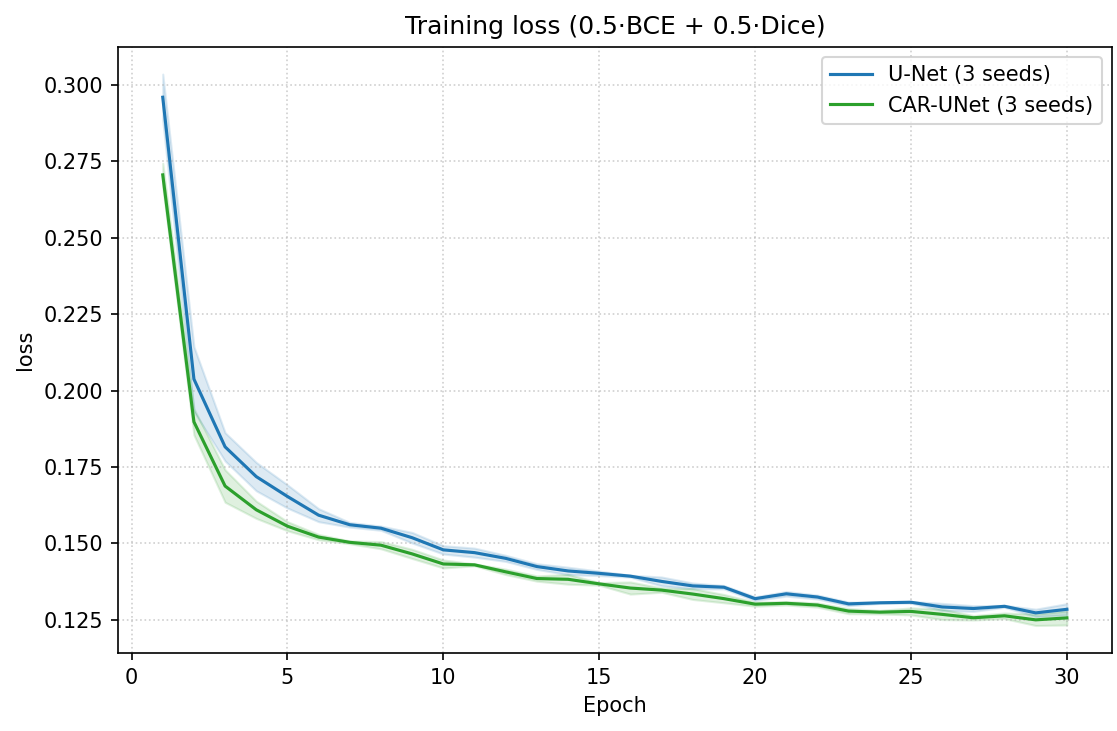
\includegraphics[width=0.48\linewidth]{curve_loss.png}\hfill
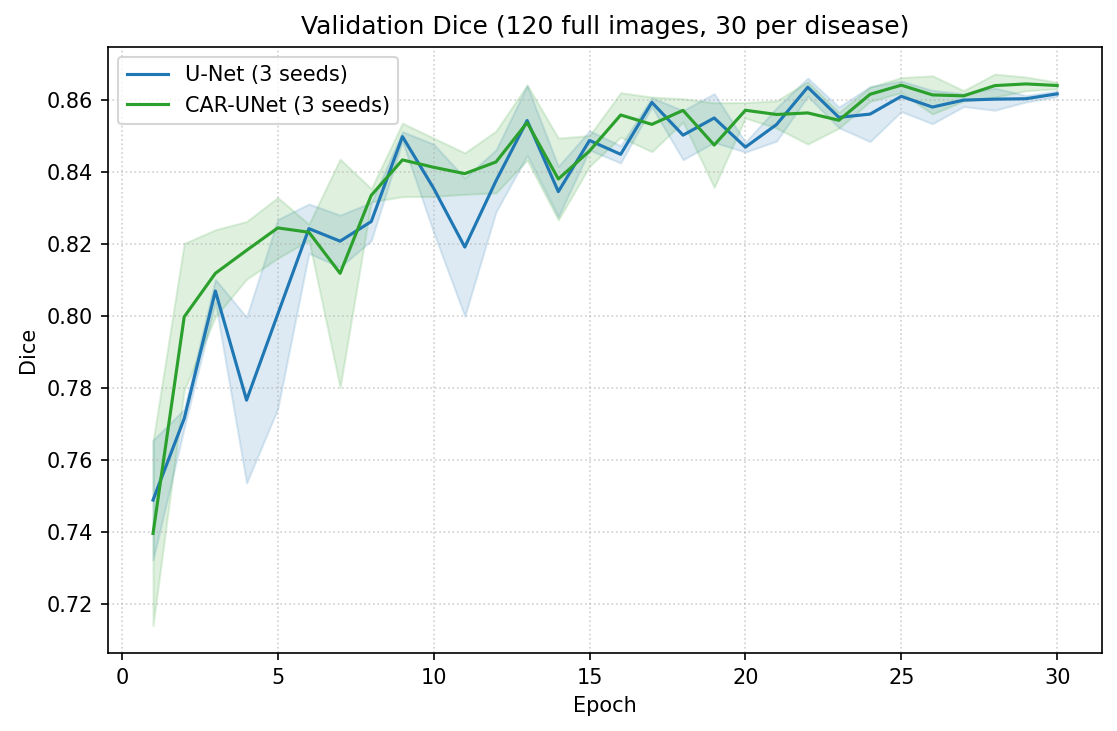
\includegraphics[width=0.48\linewidth]{curve_valdice.png}
\caption{Training loss (left) and validation Dice (right) of U-Net and CAR-UNet, mean $\pm$ standard deviation over three seeds. Validation Dice levels off at about 0.86 over the last ten epochs.}
\label{fig:curves}
\end{figure}

\subsection{Evaluation}

For every test image we count true positives (TP), false positives (FP), false negatives (FN) and true negatives (TN) inside the FOV, at a threshold of 0.5 unless stated otherwise, and compute
\begin{equation}
\begin{gathered}
\mathrm{Dice} = \frac{2\,TP}{2\,TP + FP + FN}, \qquad
\mathrm{IoU} = \frac{TP}{TP + FP + FN}, \\[4pt]
\mathrm{Sen} = \frac{TP}{TP + FN}, \qquad
\mathrm{Spe} = \frac{TN}{TN + FP}, \qquad
\mathrm{Pre} = \frac{TP}{TP + FP},
\end{gathered}
\end{equation}
together with accuracy, the area under the ROC curve (AUC) and the area under the precision--recall curve (AUC-PR). To measure connectivity we also compute the centreline Dice \citep{shit2021cldice}. With $S_P$ and $S_L$ the skeletons of the predicted and ground-truth masks $V_P$ and $V_L$,
\begin{equation}
T_{\mathrm{prec}} = \frac{|S_P \cap V_L|}{|S_P|}, \qquad
T_{\mathrm{sens}} = \frac{|S_L \cap V_P|}{|S_L|}, \qquad
\mathrm{clDice} = \frac{2\,T_{\mathrm{prec}}\,T_{\mathrm{sens}}}{T_{\mathrm{prec}} + T_{\mathrm{sens}}}.
\label{eq:cldice}
\end{equation}
Because every vessel contributes by the length of its centreline rather than its area, clDice is sensitive to missing and broken thin vessels. Metrics are averaged over the 200 test images, and we report the mean and standard deviation over the three seeds. Differences between two models are tested with the paired Wilcoxon signed-rank test \citep{wilcoxon1945} on per-image scores averaged over seeds; this test is paired and does not assume normally distributed differences.

\subsection{Proposed modifications}
\label{sec:mods}

Our replication and the paper itself reveal five weaknesses: (W1) the attention only decides \emph{which} feature channels matter, not \emph{where} the vessels are; (W2) the pixel-wise loss hardly penalises a broken thin vessel; (W3) at $512\times512$ the thinnest capillaries are lost; (W4) a fixed decision threshold of 0.5 is used; and (W5) the evaluation is weak (few images, a single run, no overlap or connectivity measures). The protocol of Section~\ref{sec:base} addresses W5. We address W1--W4 with the four modifications below, which are added cumulatively. Everything else, including data, split, seeds and training settings, is kept unchanged. Fig.~\ref{fig:arch_mod} shows the modified architecture.

\begin{figure}[t]
\centering
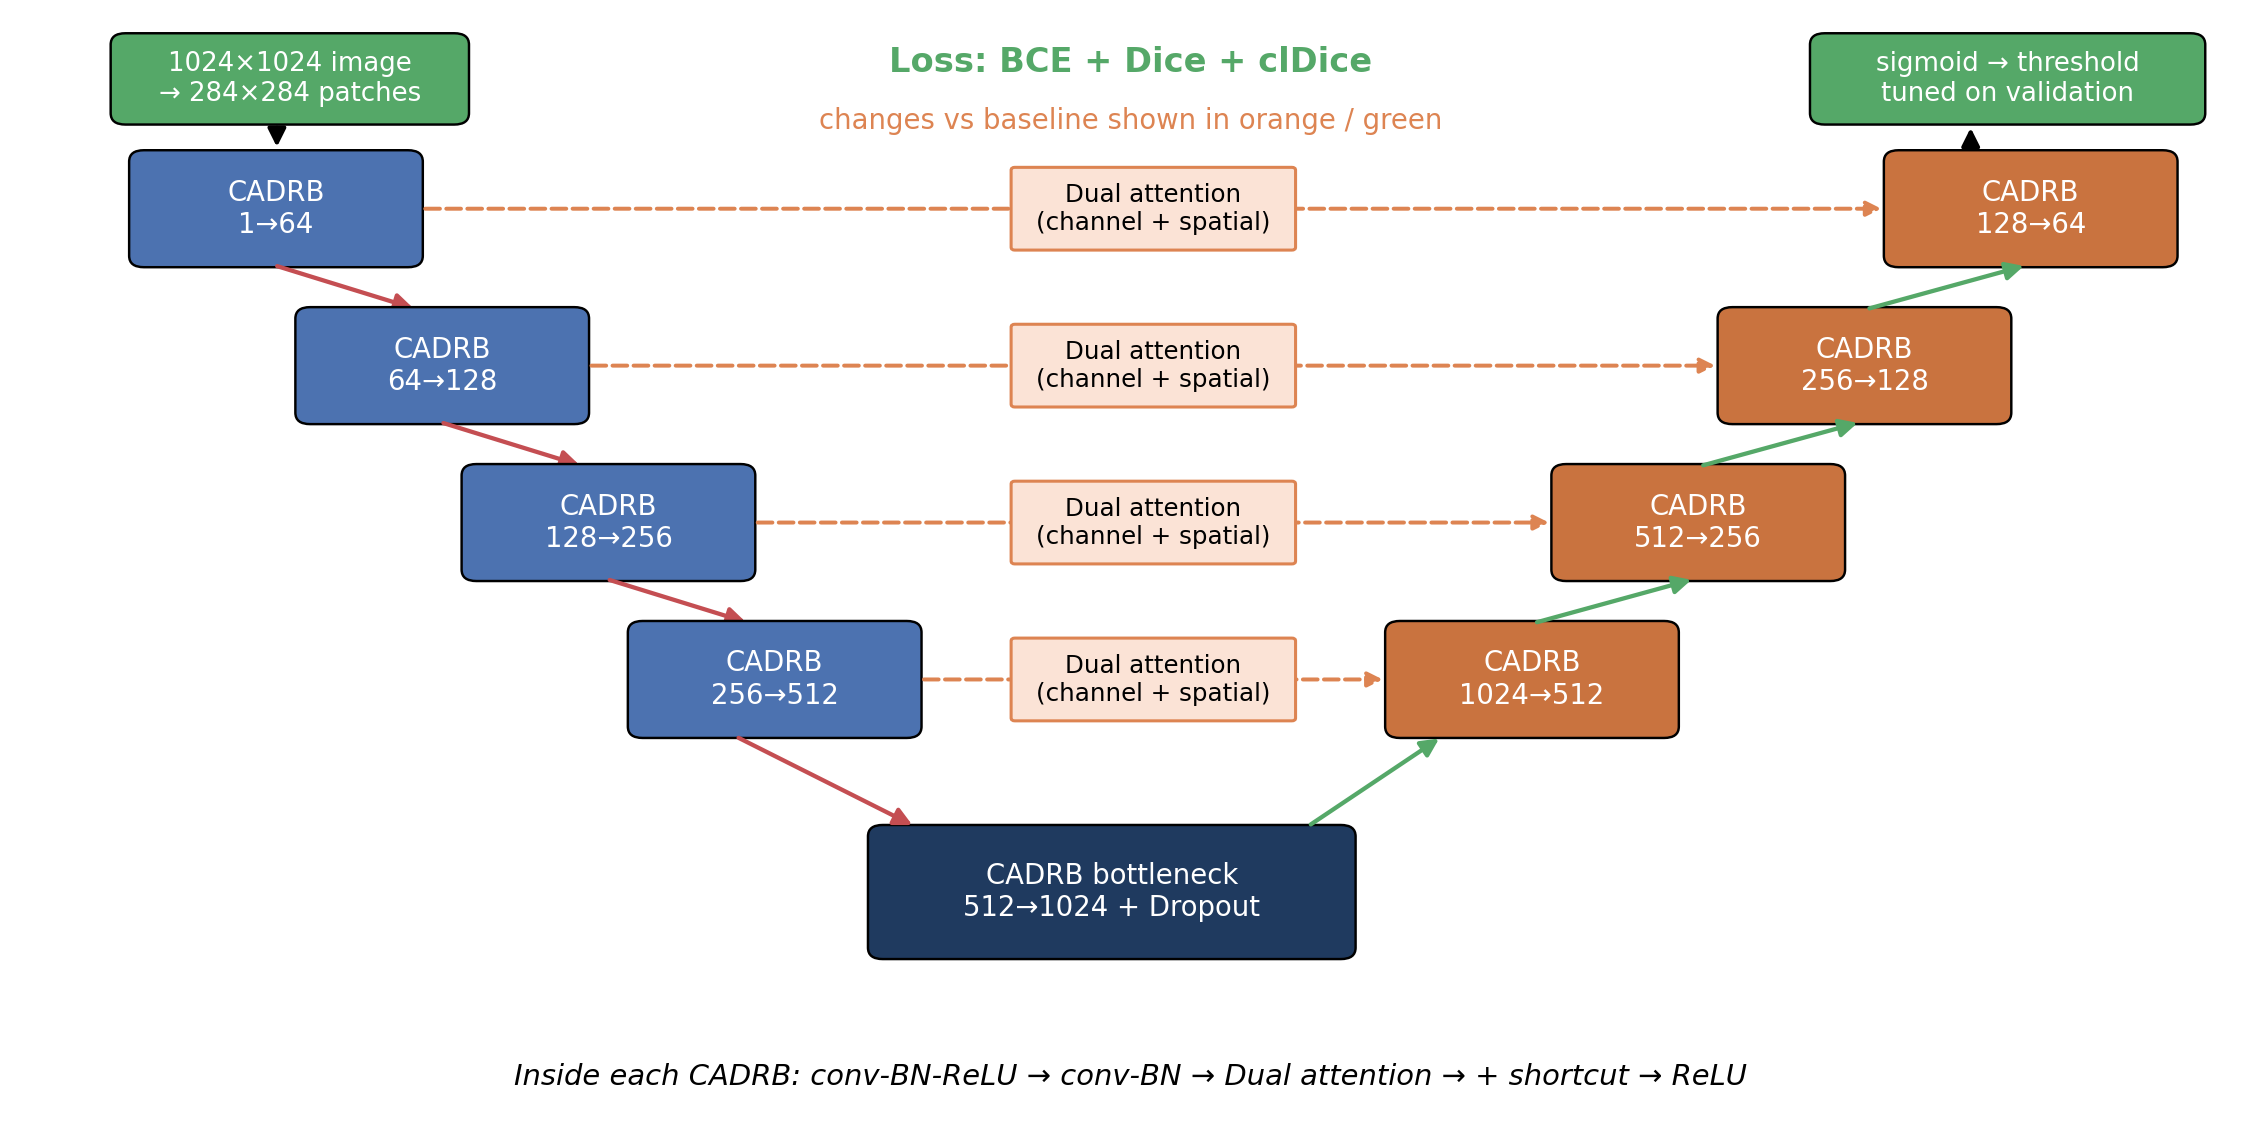
\includegraphics[width=0.92\linewidth]{arch_modified.png}
\caption{The modified architecture (changes in orange and green). Every attention module is replaced by dual attention, the input is $1024\times1024$, the loss includes clDice and the threshold is selected on the validation set.}
\label{fig:arch_mod}
\end{figure}

\paragraph{M1: Dual attention (W1).} All 13 attention modules (nine inside the residual blocks and four on the skip connections) are replaced by a dual attention block. Its first step is channel attention computed from both the average- and the max-pooled channel descriptors with a shared 1D convolution, as in the paper's own MECA formulation. Max pooling keeps the strong but spatially small responses of thin vessels, which barely change a channel's average. Its second step is spatial attention in the style of CBAM \citep{woo2018cbam}, which assigns a weight to every pixel:
\begin{align}
\mathbf{F}' &= \sigma\!\left(\mathrm{C1D}_k(\mathrm{AvgPool}(\mathbf{F})) + \mathrm{C1D}_k(\mathrm{MaxPool}(\mathbf{F}))\right) \odot \mathbf{F}, \\
\mathbf{F}'' &= \sigma\!\left(f^{7\times7}\big([\mathrm{Avg}_c(\mathbf{F}');\, \mathrm{Max}_c(\mathbf{F}')]\big)\right) \odot \mathbf{F}',
\end{align}
where $\mathrm{Avg}_c$ and $\mathrm{Max}_c$ are the mean and maximum over channels at each pixel and $f^{7\times7}$ is a $7\times7$ convolution (Fig.~\ref{fig:dual}a). All 13 blocks together add only 1,274 parameters (+0.004\%). Fig.~\ref{fig:dual}b shows that the learned spatial attention map is clearly organised around the vessel tree, including many thin branches; the block therefore re-weights the features according to vessel location, which channel attention alone cannot do.

\begin{figure}[t]
\centering
\begin{minipage}[b]{0.33\linewidth}\centering
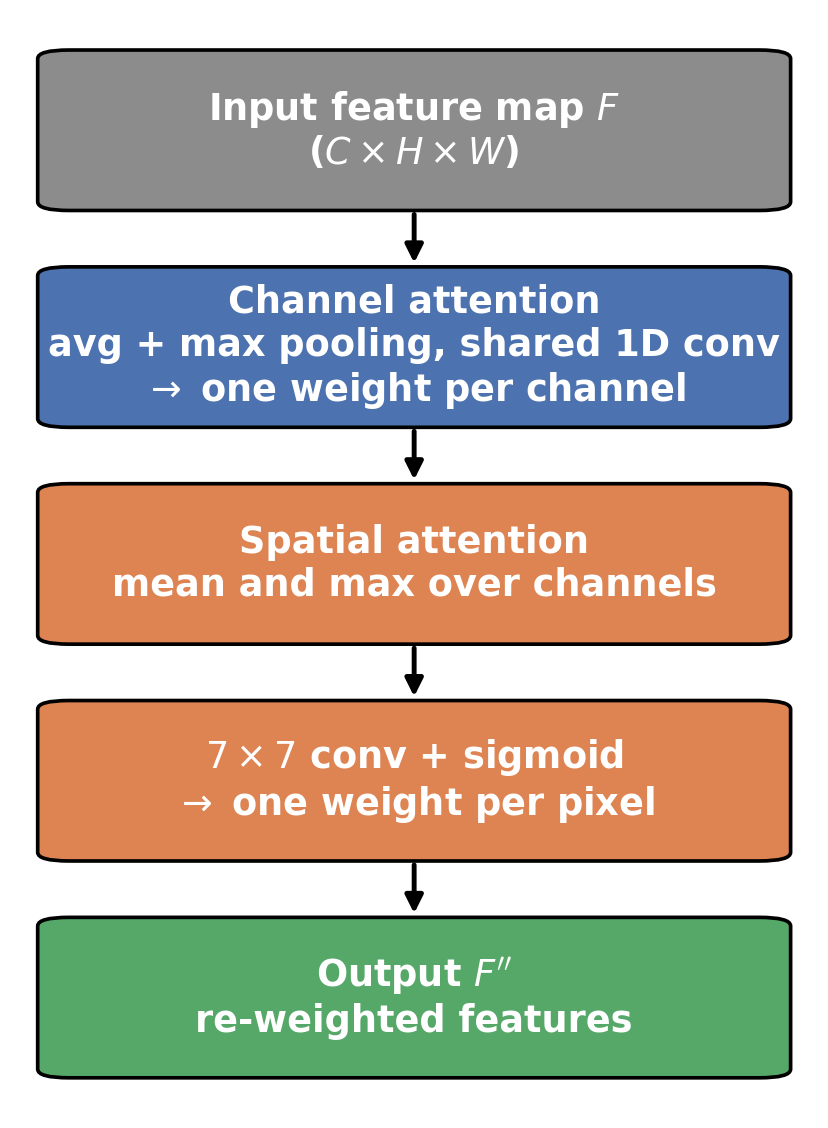
\includegraphics[width=\linewidth]{dual_attention_block.png}\\[2pt]{\small (a)}
\end{minipage}\hfill
\begin{minipage}[b]{0.62\linewidth}\centering
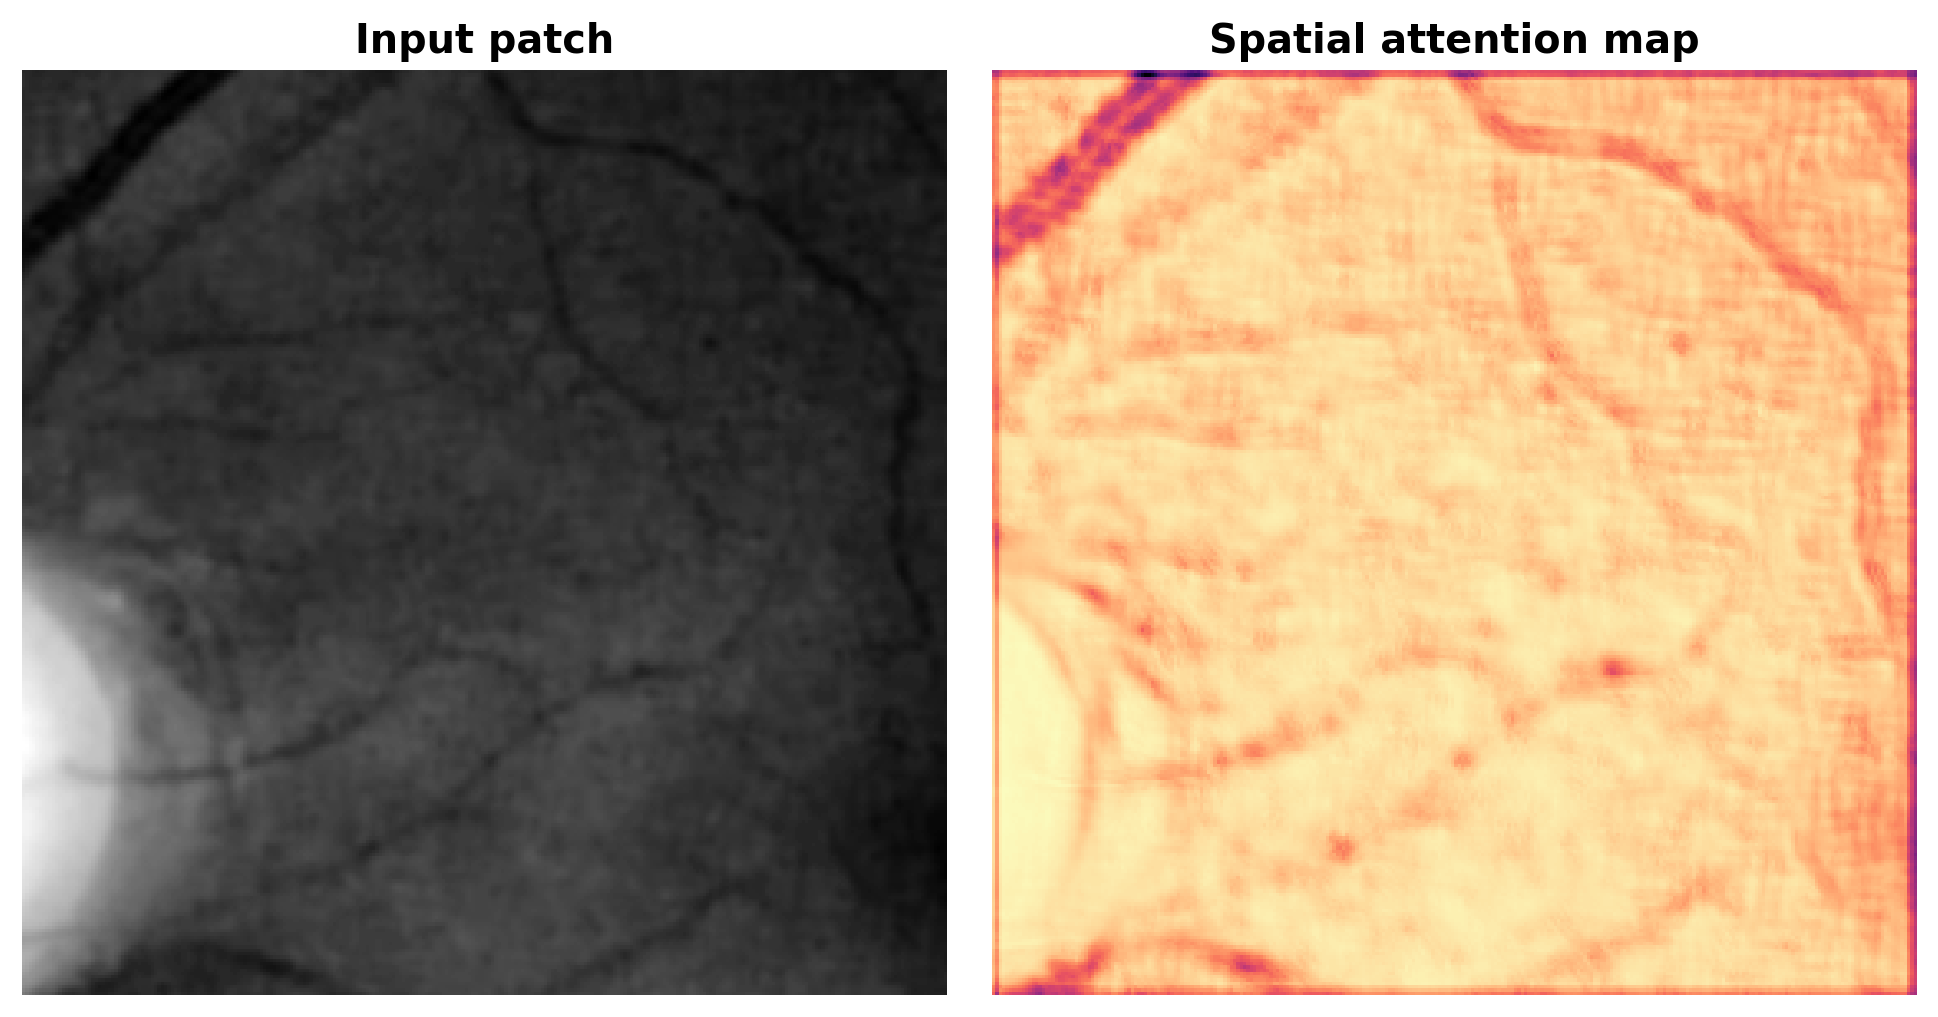
\includegraphics[width=\linewidth]{ev_attention.png}\\[2pt]{\small (b)}
\end{minipage}
\caption{Dual attention. (a) Structure of the block: channel attention from average and max pooling, followed by spatial attention that assigns one weight to every pixel. (b) A preprocessed input patch (glaucoma test image, $1024\times1024$ model) and the spatial attention map of the first encoder block (light = high weight). The vessel tree is clearly visible in the map; in this early block, vessel pixels receive slightly lower weights than the background (mean 0.85 versus 0.90).}
\label{fig:dual}
\end{figure}

\paragraph{M2: clDice loss (W2).} We add the clDice loss \citep{shit2021cldice}, $\mathcal{L}_{\mathrm{clDice}} = 1 - \mathrm{clDice}$, computed with a differentiable soft skeleton (iterated soft erosion and dilation) on the predicted probabilities:
\begin{equation}
\mathcal{L} = 0.5\,\mathcal{L}_{\mathrm{BCE}} + 0.5\left[(1-\alpha)\,\mathcal{L}_{\mathrm{Dice}} + \alpha\,\mathcal{L}_{\mathrm{clDice}}\right], \qquad \alpha = 0.5.
\end{equation}
On a synthetic test image, cutting a thin vessel (20 pixels) raises the clDice loss 4.5 times more than the Dice loss, whereas trimming the end of a thick vessel costs less under clDice, because the vessel stays connected (Fig.~\ref{fig:evidence}a).

\paragraph{M3: Higher working resolution (W3).} The improved model is trained and applied at $1024\times1024$ pixels. A capillary that is a fraction of a pixel wide at $512\times512$ becomes about twice as wide and survives the resizing (Fig.~\ref{fig:evidence}b). For a fair comparison, the $1024\times1024$ prediction is downsampled and scored on exactly the same $512\times512$ ground truth as the baseline. In addition, we score all models against the $1024\times1024$ ground truth, upsampling the predictions of the $512\times512$ models. The soft skeleton uses 20 instead of 10 iterations because vessels are twice as wide in pixels. The number of training patches per epoch is unchanged.

\paragraph{M4: Validation-selected threshold (W4).} For each trained model we evaluate thresholds from 0.20 to 0.80 (step 0.02) on the validation set and keep the one with the highest validation Dice. We also tested test-time augmentation (TTA), averaging the predictions on four flipped copies of each image, and let the validation set decide whether to use it.

\begin{figure}[t]
\centering
\begin{minipage}[t]{0.48\linewidth}\centering
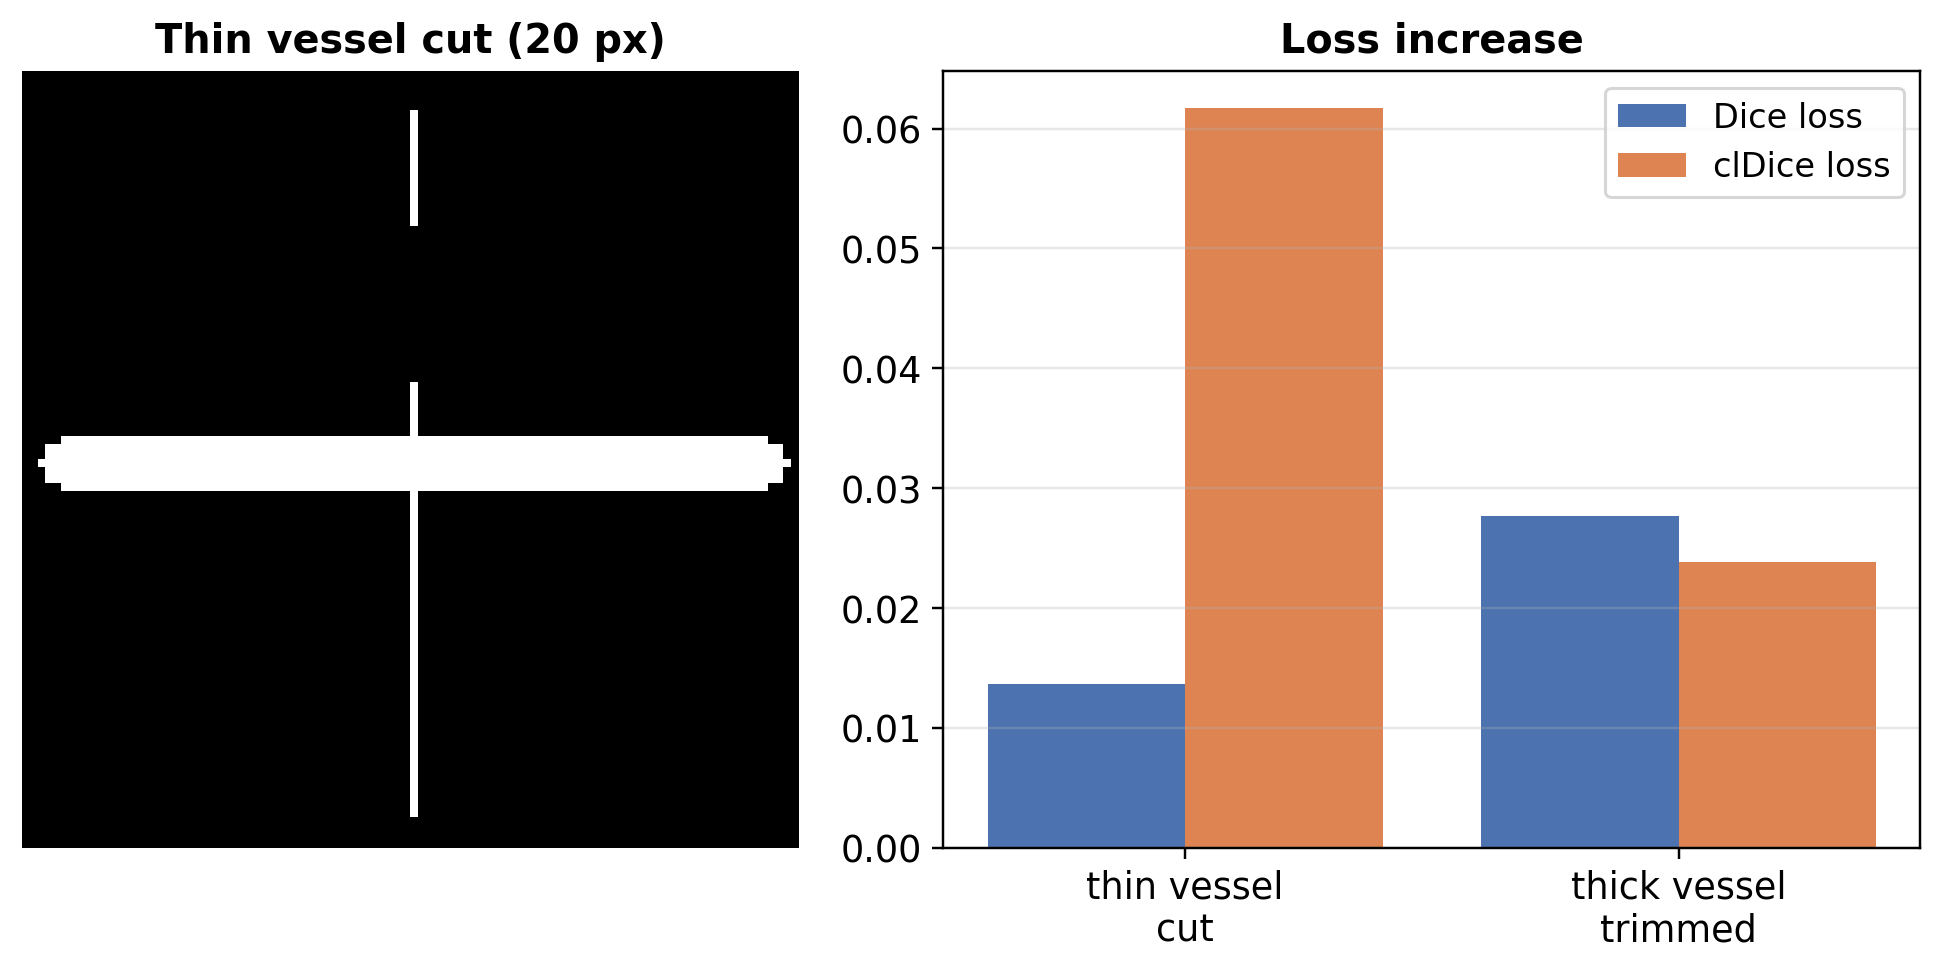
\includegraphics[width=\linewidth]{ev_cldice.png}\\[2pt]{\small (a)}
\end{minipage}\hfill
\begin{minipage}[t]{0.48\linewidth}\centering
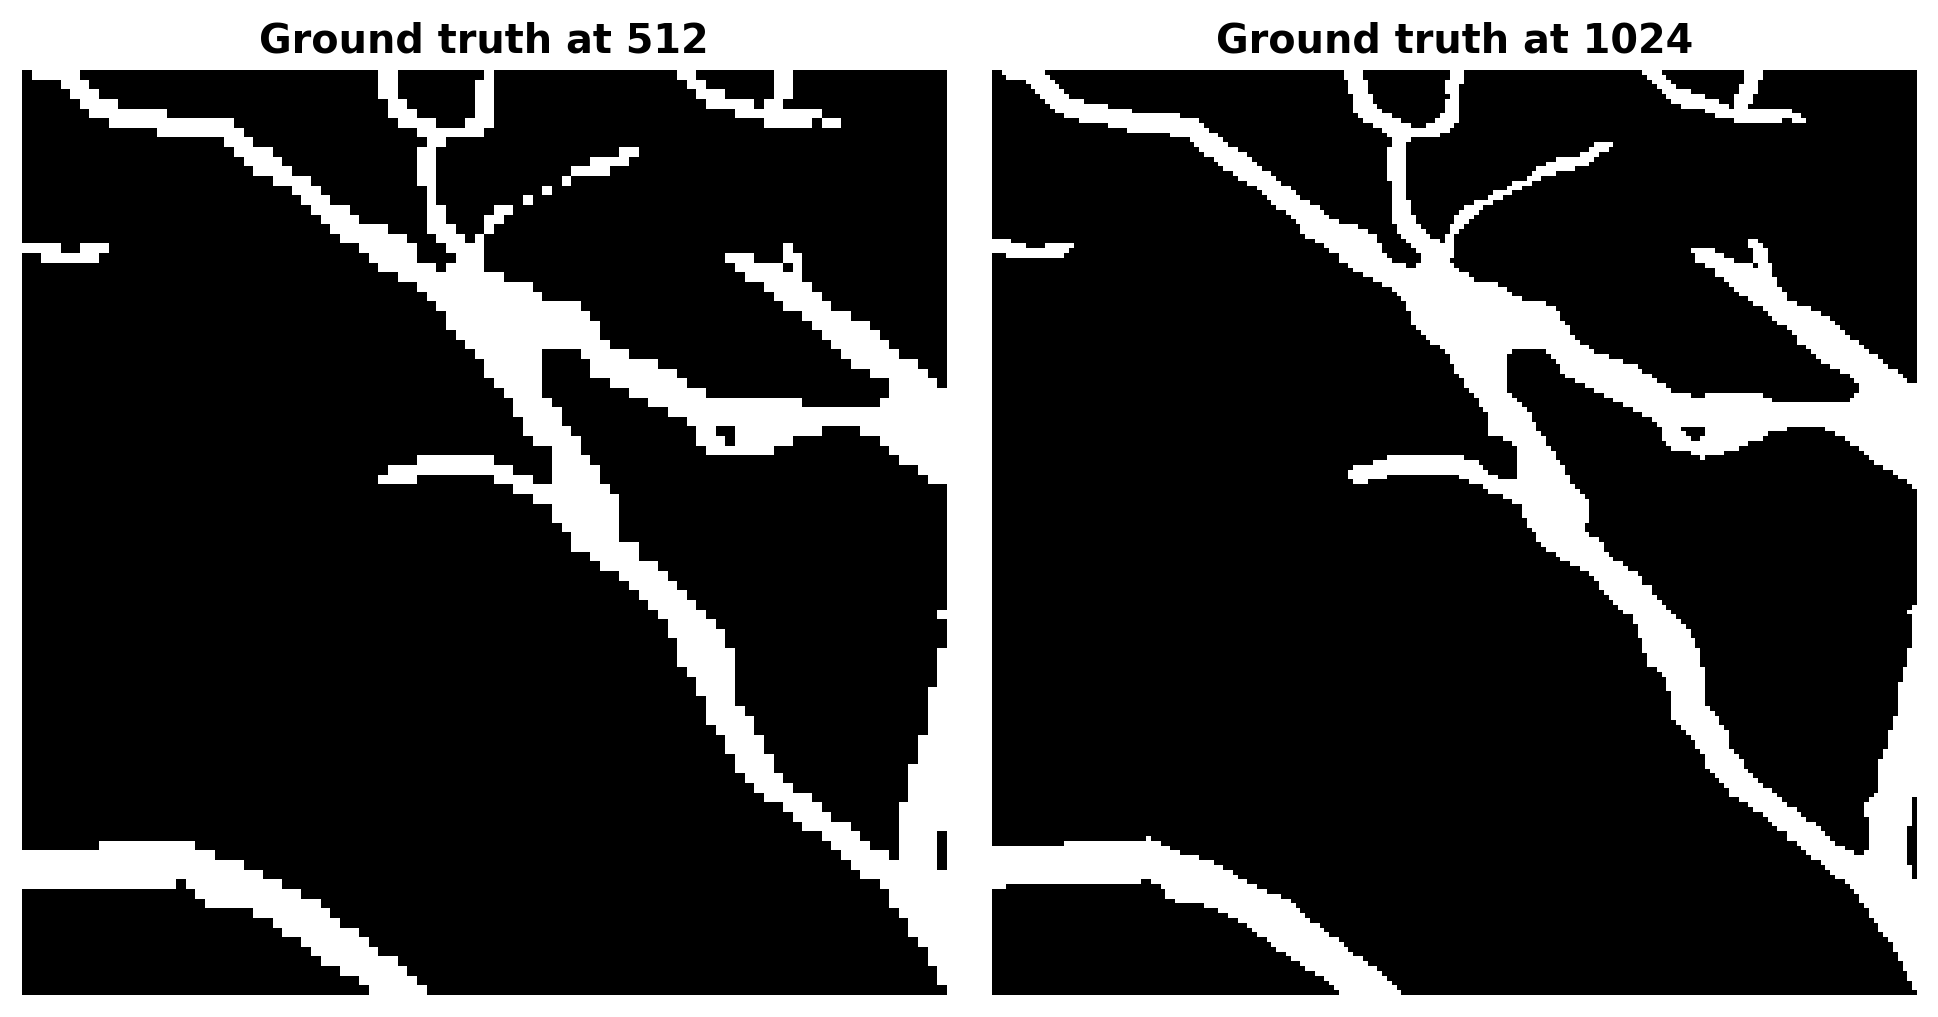
\includegraphics[width=\linewidth]{ev_resolution.png}\\[2pt]{\small (b)}
\end{minipage}
\caption{Motivation for M2 and M3. (a) Synthetic test: cutting a 20-pixel piece out of a thin vessel raises the clDice loss 4.5 times more than the Dice loss, while trimming a thick vessel costs about the same under both. (b) The same ground-truth region at $512\times512$ and $1024\times1024$: thin vessels that are fragmented at $512\times512$ are continuous at $1024\times1024$.}
\label{fig:evidence}
\end{figure}

%% ===============================================================================
\section{Results}
\label{sec:results}

\subsection{Comparison with the replicated baseline}

Table~\ref{tab:main} compares the replicated CAR-UNet with the improved model on the same split, with the same seeds and training settings. The improved model is better on Dice (+0.54 points), IoU (+0.83), sensitivity (+1.55), accuracy, AUC, AUC-PR and clDice (+1.25), and all of these differences are statistically significant. It is better in every one of the three seeds: Dice gains of +0.55, +0.78 and +0.30 points, and clDice gains of +0.68, +1.82 and +1.24 points. Precision ($-0.40$) and specificity ($-0.09$) are slightly lower, which is the expected cost of detecting more vessel pixels. Fig.~\ref{fig:change} summarises the change in every metric.

\begin{table}[t]
\caption{Replicated baseline versus improved model on the 200 FIVES test images (mean $\pm$ standard deviation over three seeds). Change in percentage points; \emph{better on}: test images on which the improved model scores higher; $p$: paired Wilcoxon signed-rank test.}
\label{tab:main}
\centering
\begin{tabular}{lccccc}
\toprule
Metric & Baseline (CAR-UNet) & Improved & Change & Better on & $p$ \\
\midrule
Dice & $0.8382 \pm 0.0031$ & $\mathbf{0.8436 \pm 0.0027}$ & +0.54 & 140/200 & $4.8\times10^{-10}$ \\
IoU & $0.7295 \pm 0.0043$ & $\mathbf{0.7379 \pm 0.0039}$ & +0.83 & 140/200 & $2.0\times10^{-10}$ \\
Sensitivity & $0.8310 \pm 0.0126$ & $\mathbf{0.8465 \pm 0.0011}$ & +1.55 & 159/200 & $7.4\times10^{-19}$ \\
Specificity & $\mathbf{0.9855 \pm 0.0018}$ & $0.9846 \pm 0.0008$ & $-$0.09 & 51/200 & $6.3\times10^{-15}$ \\
Precision & $\mathbf{0.8557 \pm 0.0151}$ & $0.8516 \pm 0.0054$ & $-$0.40 & 68/200 & $9.6\times10^{-8}$ \\
Accuracy & $0.9728 \pm 0.0007$ & $\mathbf{0.9737 \pm 0.0006}$ & +0.09 & 130/200 & $1.8\times10^{-8}$ \\
AUC & $0.9860 \pm 0.0014$ & $\mathbf{0.9878 \pm 0.0003}$ & +0.17 & 168/200 & $1.4\times10^{-21}$ \\
AUC-PR & $0.9202 \pm 0.0044$ & $\mathbf{0.9260 \pm 0.0006}$ & +0.58 & 163/200 & $9.4\times10^{-18}$ \\
clDice & $0.8626 \pm 0.0057$ & $\mathbf{0.8751 \pm 0.0005}$ & +1.25 & 175/200 & $5.3\times10^{-25}$ \\
\bottomrule
\end{tabular}
\end{table}

\begin{figure}[t]
\centering
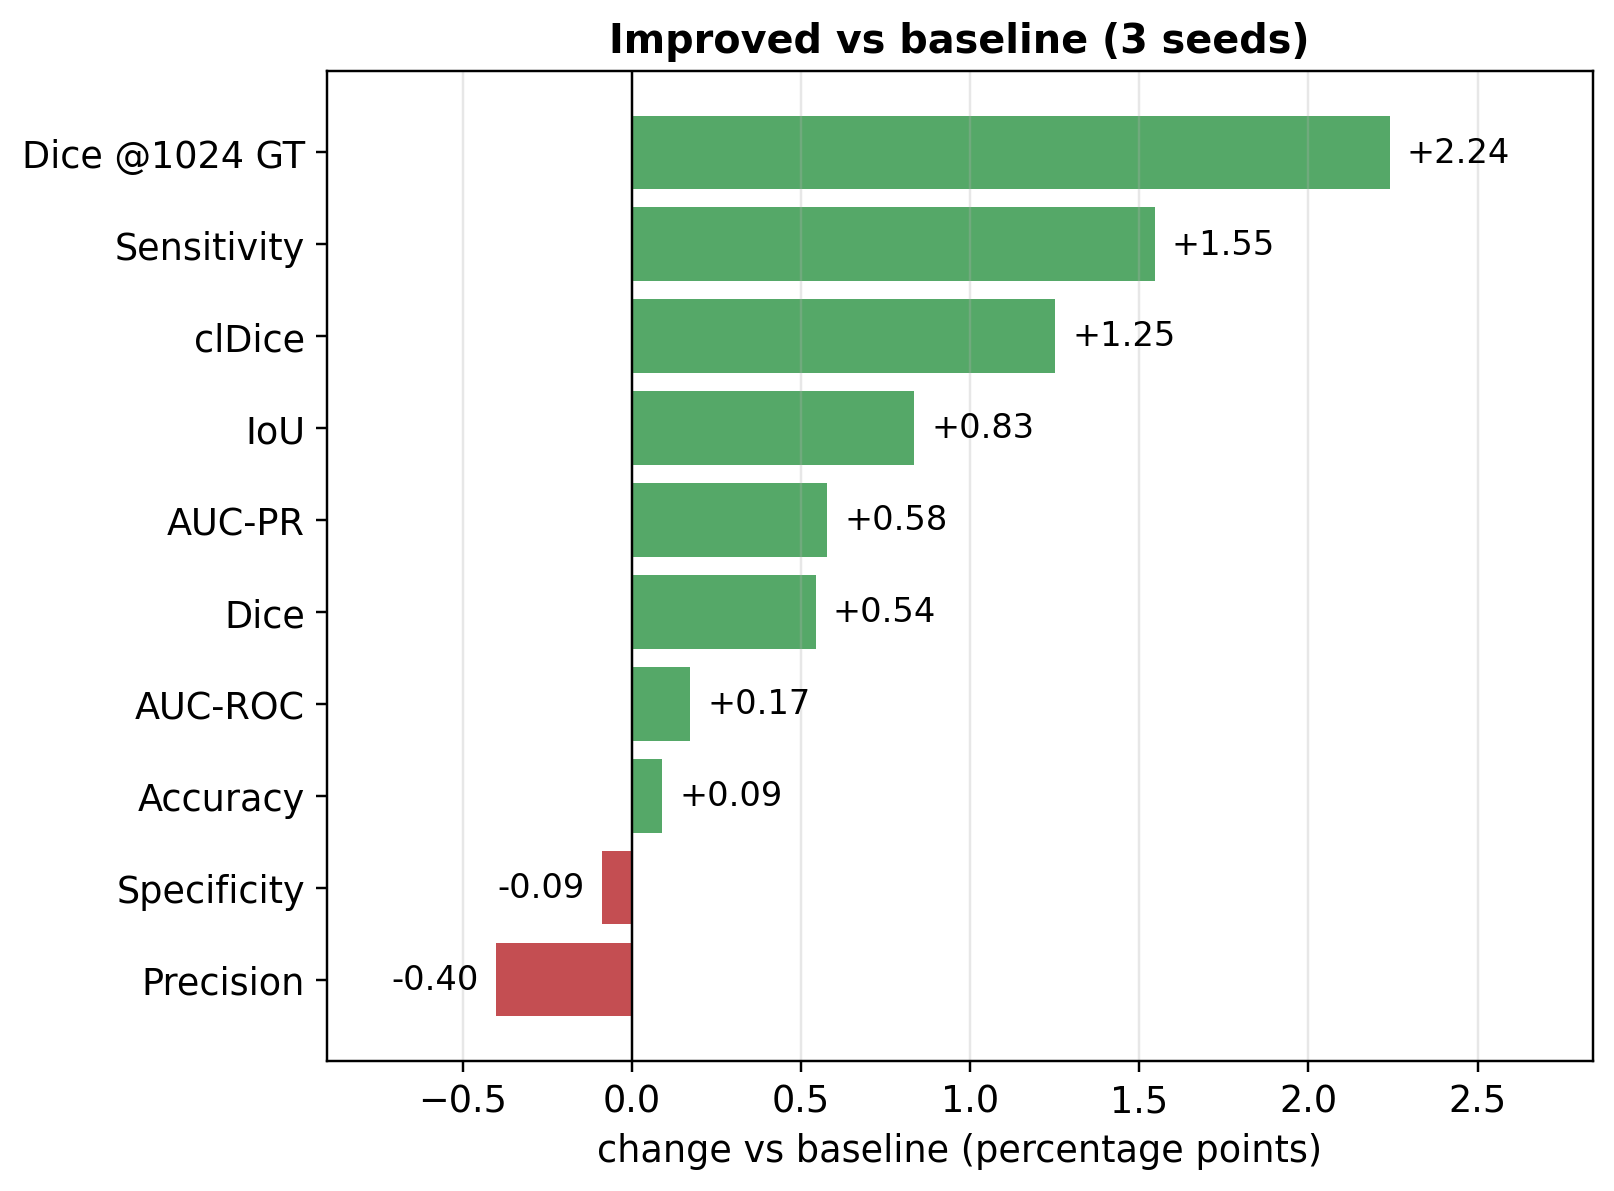
\includegraphics[width=0.6\linewidth]{change_per_metric.png}
\caption{Change of every metric from the replicated baseline to the improved model (percentage points, three seeds). Green: the improved model is better.}
\label{fig:change}
\end{figure}

\subsection{Ablation study}

Table~\ref{tab:ablation} and Fig.~\ref{fig:ablation} add the modifications one at a time. Each component has a distinct effect. Dual attention raises Dice by 0.26 points, with a higher Dice on 167/200 images ($p = 2\times10^{-19}$), mainly by removing false detections (precision +0.63 points); it also gives the most stable results across seeds. The clDice loss strongly improves connectivity (+0.88 clDice points over dual attention, better on 191/200 images, $p = 2\times10^{-32}$) and sensitivity (+1.24 points), but at the default threshold it also adds false detections, so Dice stays level. Moving to $1024\times1024$ raises Dice by 0.40 points over the same model at $512\times512$ (better on 150/200 images, $p = 2\times10^{-11}$) and precision by 2.0 points, at the cost of some sensitivity. Finally, the validation-selected threshold (0.44--0.48 for the three high-resolution models) converts this precision into recall: sensitivity rises by 1.39 points and Dice by 0.15 points (better on 148/200 images, $p = 5\times10^{-17}$).

\begin{table}[t]
\caption{Ablation study: modifications added one at a time to the replicated CAR-UNet (200 test images, three seeds; Dice: mean $\pm$ standard deviation).}
\label{tab:ablation}
\centering
\begin{tabular}{lccccc}
\toprule
Model & Dice & IoU & Sensitivity & Precision & clDice \\
\midrule
U-Net (reference) & $0.8344 \pm 0.0034$ & 0.7246 & 0.8247 & 0.8573 & 0.8593 \\
CAR-UNet (replicated baseline) & $0.8382 \pm 0.0031$ & 0.7295 & 0.8310 & 0.8557 & 0.8626 \\
\quad + M1 dual attention & $0.8408 \pm 0.0021$ & 0.7339 & 0.8308 & 0.8620 & 0.8631 \\
\quad + M2 clDice loss & $0.8382 \pm 0.0050$ & 0.7293 & 0.8432 & 0.8430 & 0.8718 \\
\quad + M3 $1024\times1024$ input & $0.8421 \pm 0.0028$ & 0.7359 & 0.8326 & \textbf{0.8632} & 0.8742 \\
\quad + M4 tuned threshold (final) & $\mathbf{0.8436 \pm 0.0027}$ & \textbf{0.7379} & \textbf{0.8465} & 0.8516 & \textbf{0.8751} \\
\bottomrule
\end{tabular}
\end{table}

\begin{figure}[t]
\centering
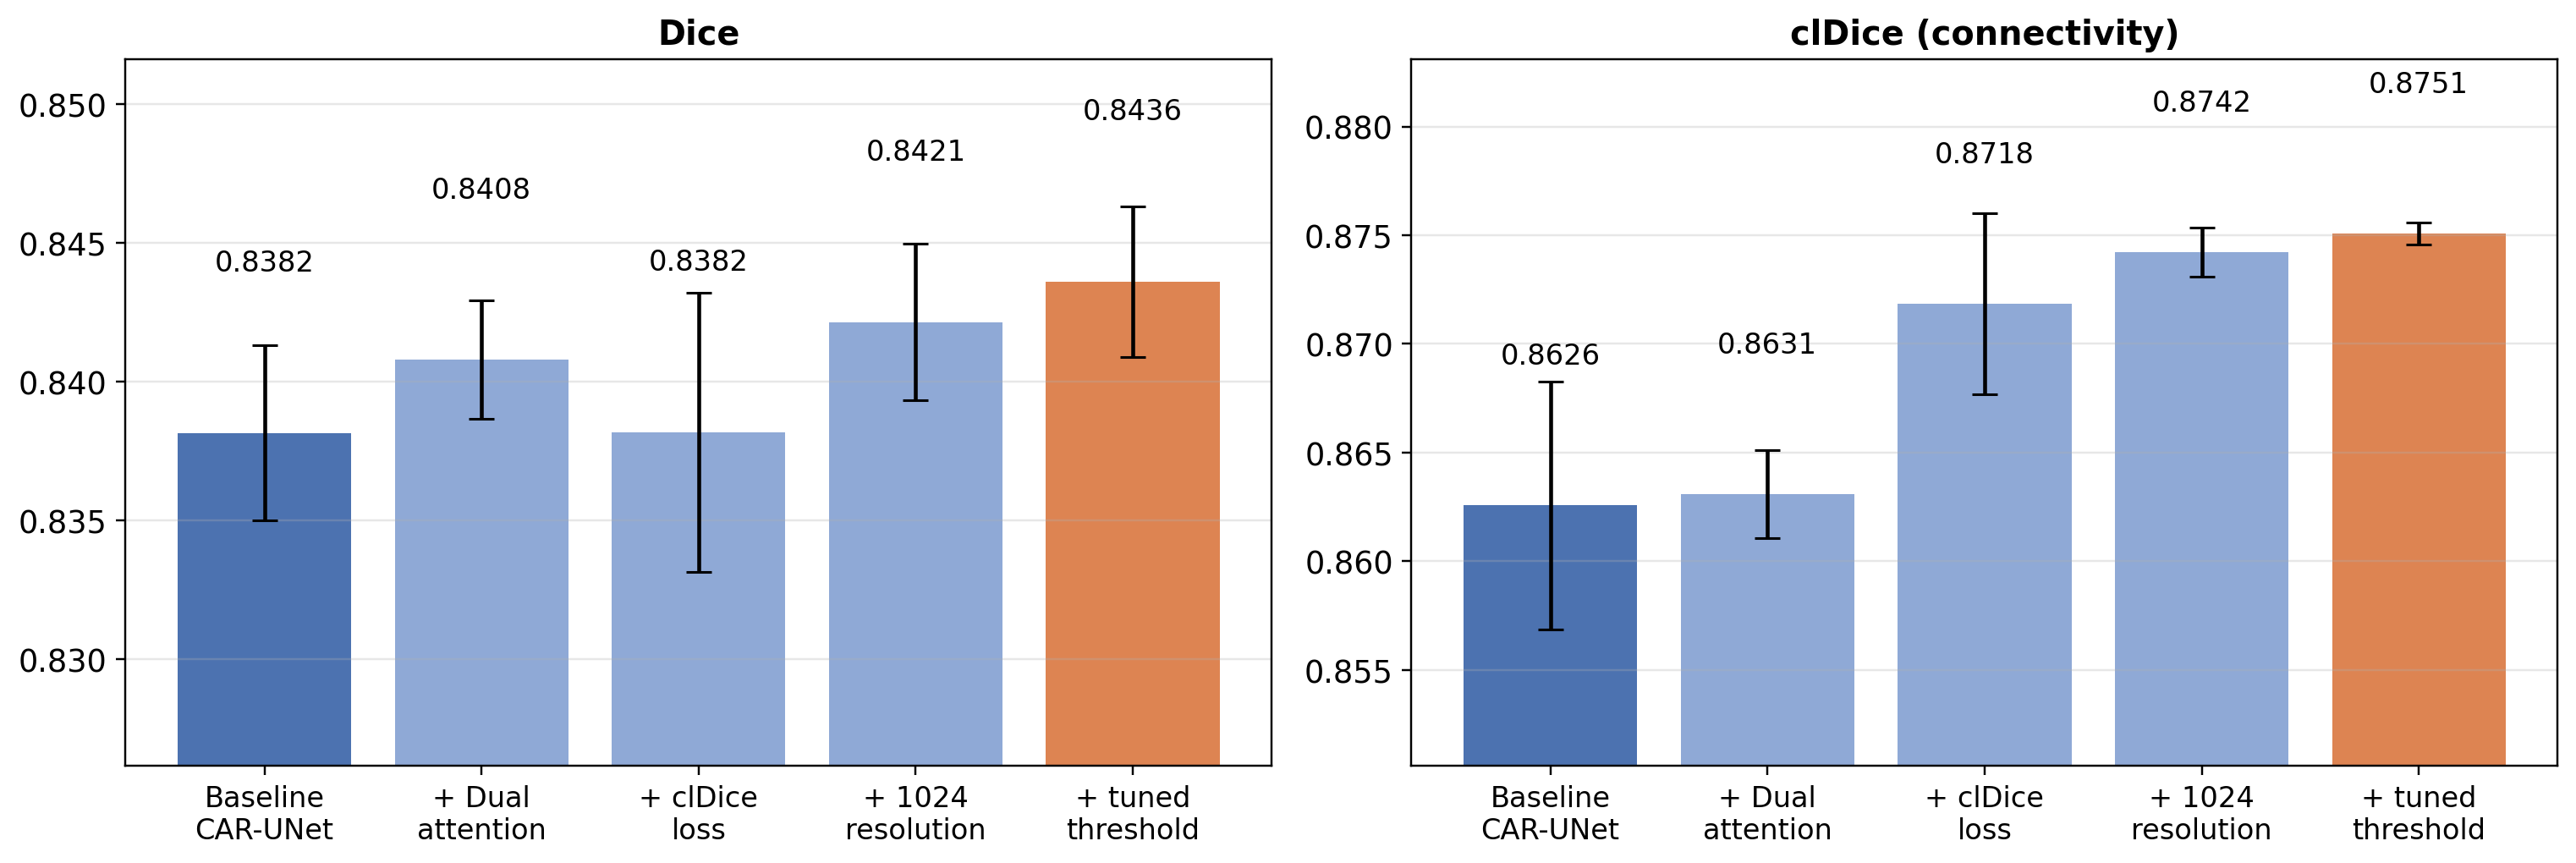
\includegraphics[width=0.92\linewidth]{ablation.png}
\caption{Ablation: Dice (left) and clDice (right) after each modification, mean $\pm$ standard deviation over three seeds.}
\label{fig:ablation}
\end{figure}

\subsection{Per-disease results}

Table~\ref{tab:disease} breaks the results down by disease group. Connectivity improves in every group. Dice improves for AMD, DR and normal eyes, most strongly for normal eyes (+1.78 points), but not for glaucoma ($-0.11$ points), which remains the hardest group for both models. Glaucoma images in FIVES contain the fewest annotated vessels (8.5\% of the field of view, against 11.4\% for normal eyes), so each missed vessel weighs more. The group also contains the two test images on which every model fails (Dice below 0.1): very hazy, dark images whose expert masks contain only 0.7\% and 1.7\% vessel pixels, because few vessels are visible at all. We kept both images in the test set, since excluding hard cases would inflate the results.

\begin{table}[t]
\caption{Dice and clDice per disease group (50 test images each, three seeds).}
\label{tab:disease}
\centering
\begin{tabular}{lcccccc}
\toprule
 & \multicolumn{3}{c}{Dice} & \multicolumn{3}{c}{clDice} \\
\cmidrule(lr){2-4}\cmidrule(lr){5-7}
Disease & Baseline & Improved & Change & Baseline & Improved & Change \\
\midrule
AMD & 0.8643 & \textbf{0.8671} & +0.28 & 0.8884 & \textbf{0.8978} & +0.94 \\
DR & 0.8562 & \textbf{0.8585} & +0.22 & 0.8807 & \textbf{0.8895} & +0.88 \\
Glaucoma & \textbf{0.7958} & 0.7947 & $-$0.11 & 0.8178 & \textbf{0.8227} & +0.49 \\
Normal & 0.8363 & \textbf{0.8541} & +1.78 & 0.8635 & \textbf{0.8904} & +2.69 \\
\bottomrule
\end{tabular}
\end{table}

\subsection{Thin vessels}

Two measurements focus on the thin vessels that motivated this work. First, the fraction of thin-vessel pixels (vessel radius $\le 1.5$ pixels in the ground truth) found by the model rises from 0.781 to 0.788 for seed 0, and is higher on 139 of 200 images ($p = 2.7\times10^{-7}$). Second, when all models are scored against the $1024\times1024$ ground truth, in which thin vessels are much better represented, the $1024\times1024$ model reaches a Dice of $0.8796 \pm 0.0015$ and a clDice of 0.8972 (threshold 0.5), against 0.8572 and 0.8791 for the replicated CAR-UNet and 0.8599 and 0.8895 for the same model trained at $512\times512$. Higher resolution therefore accounts for most of the gain at full resolution (+2.2 Dice points over the baseline).

\subsection{Qualitative results}

Fig.~\ref{fig:qualitative} shows the median test image of each disease group processed by both models. At full scale the differences are subtle, since both models trace the main vessels well, but the zoomed error maps reveal them clearly: the improved model leaves fewer missed thin branches (blue) and keeps them connected, at the cost of a few additional false-positive pixels (red) along vessel borders. The improved model scores higher on all four examples, including the glaucoma image, although on average it does not improve Dice for that group (Table~\ref{tab:disease}).

\begin{figure}[t]
\centering
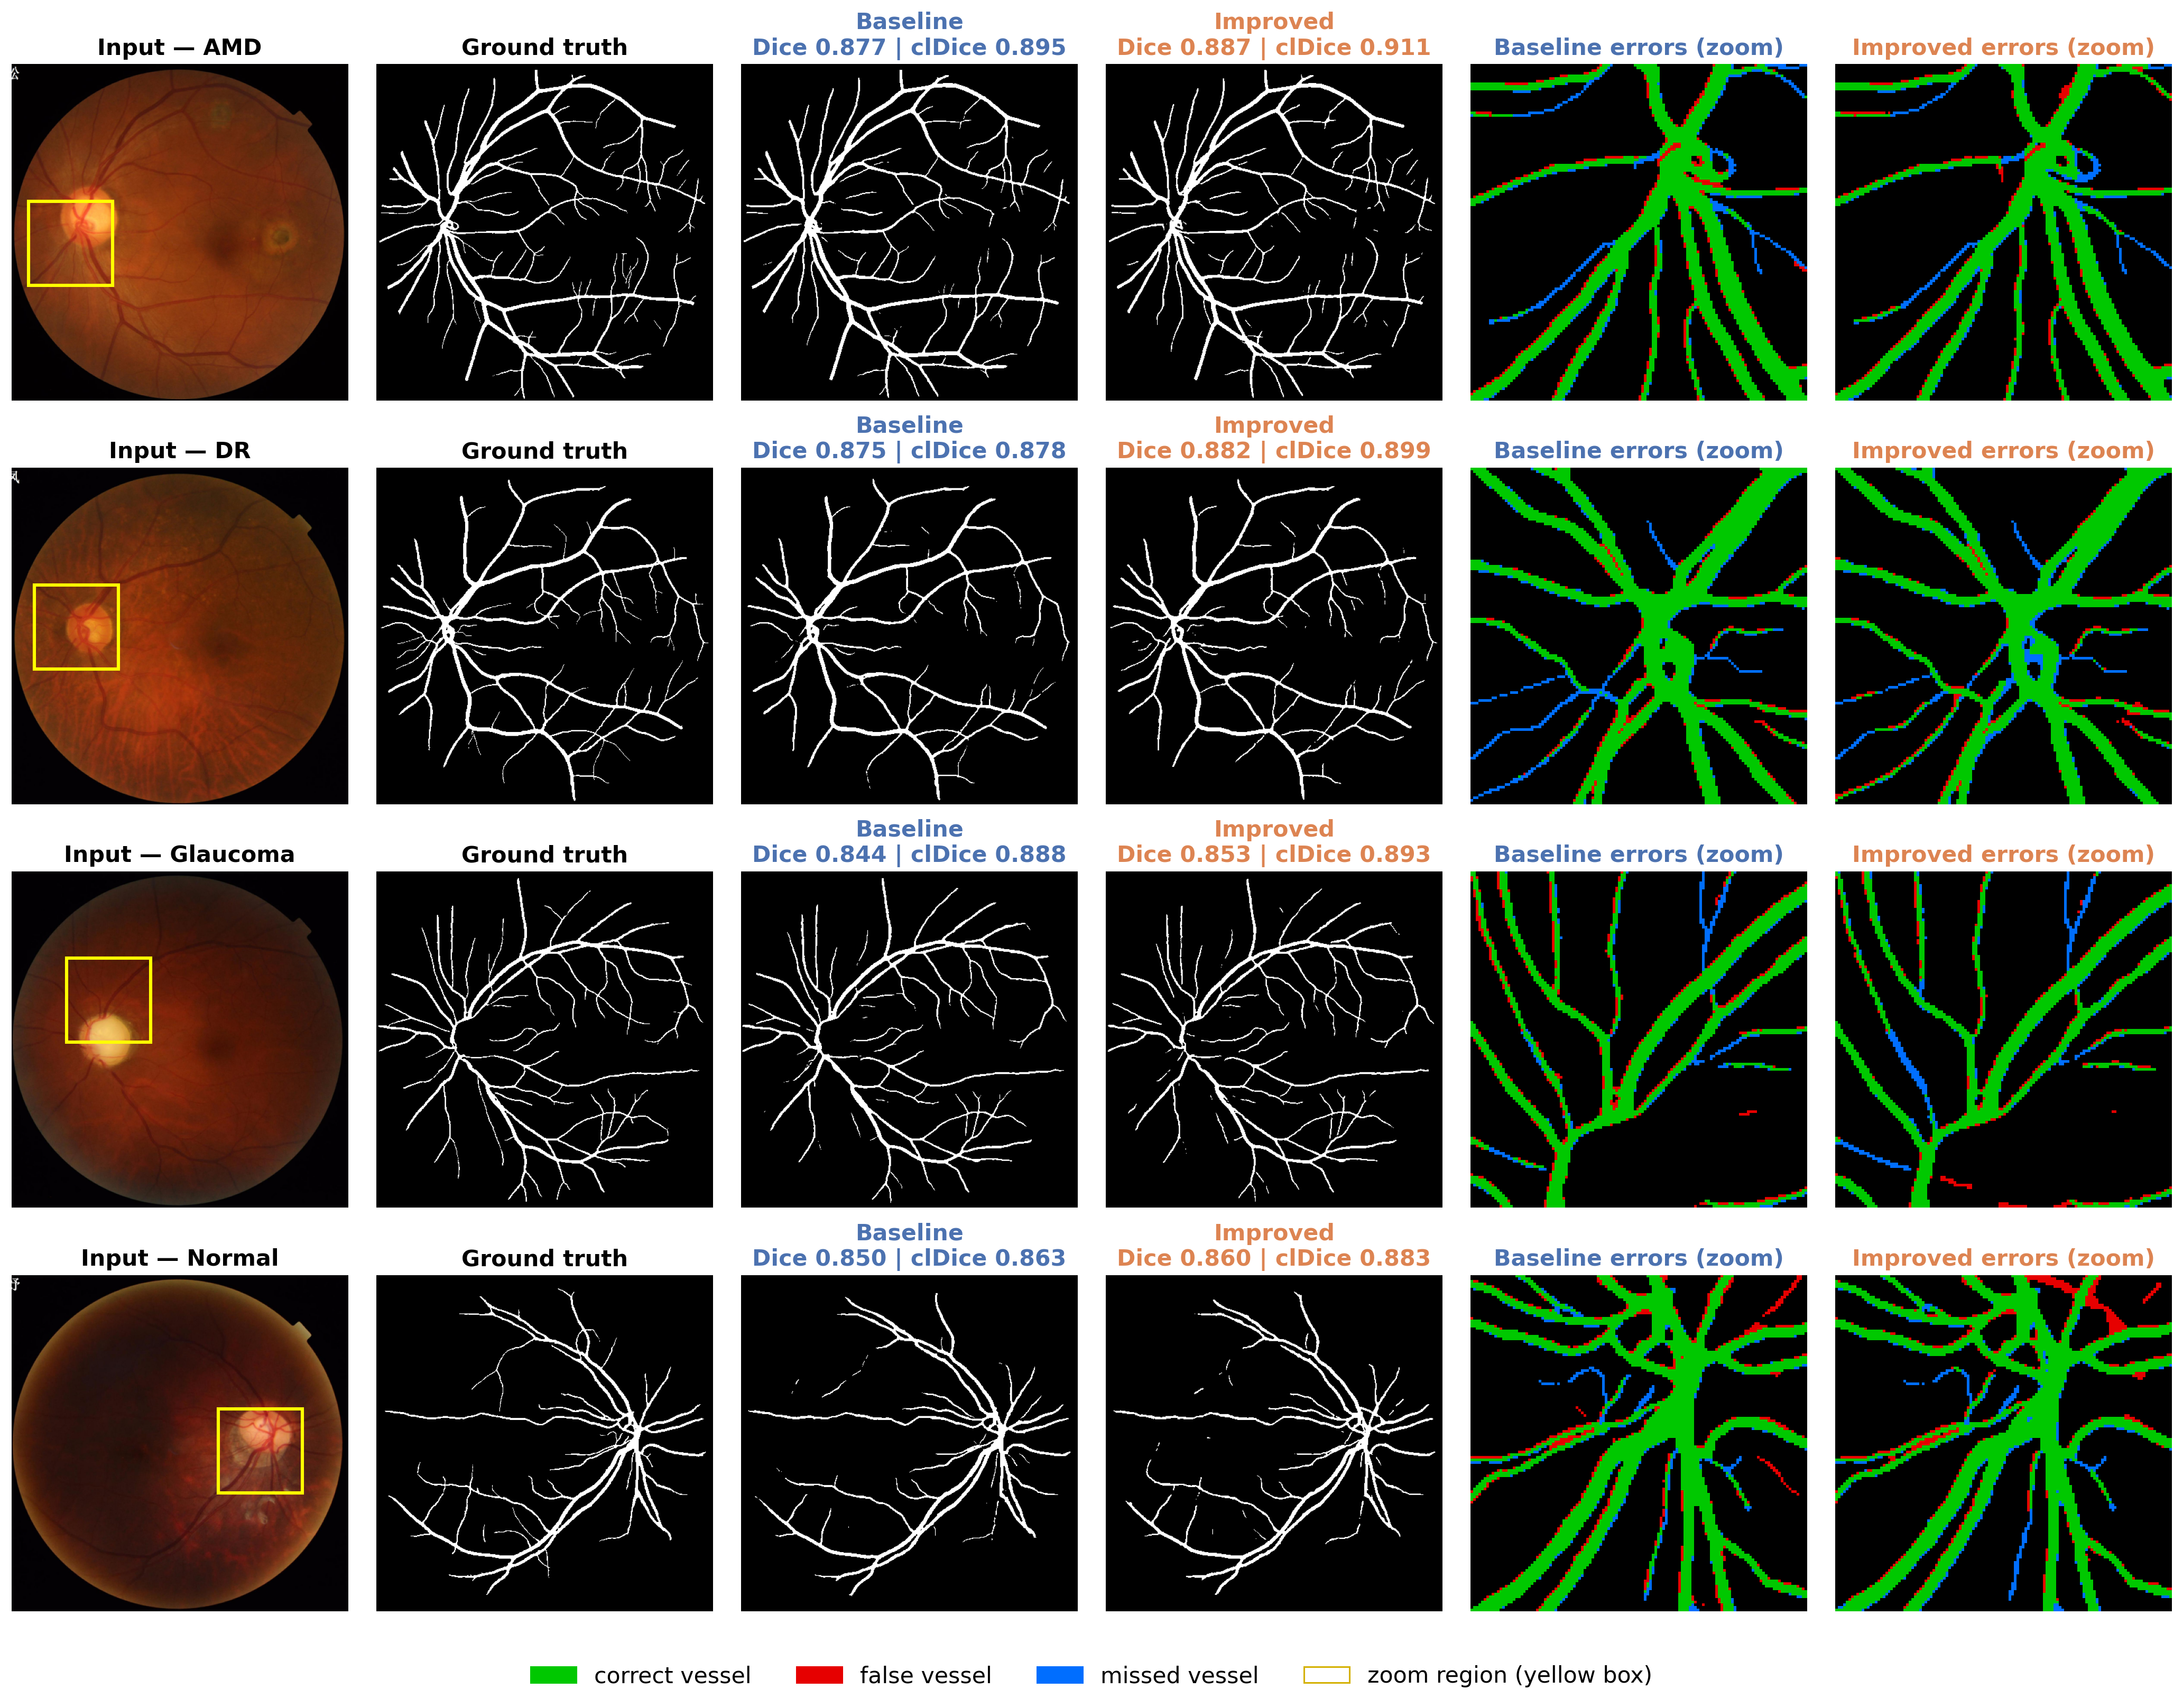
\includegraphics[width=\linewidth]{compare_all_diseases.png}
\caption{Qualitative comparison on one test image per disease group (the image with the median baseline Dice of its group, not hand-picked; seed 0). Columns: input (the yellow box marks the $128\times128$ region with the most thin vessels), ground truth, baseline and improved predictions, and zoomed error maps of both models (green: correct vessel, red: false vessel, blue: missed vessel).}
\label{fig:qualitative}
\end{figure}

\subsection{What did not work}

Test-time augmentation lowered Dice for every model at the default threshold, by 0.2 to 0.7 points. A diagnostic on four validation images showed why: for one model, the individual predictions on flipped images were up to 2.6 Dice points worse than on the original image (0.868 original, 0.864 horizontal flip, 0.851 vertical flip, 0.842 both). Averaging them therefore mixes in weaker predictions. The models are not fully orientation-invariant, even though flips were used during training. Because the prediction setting is selected on the validation set, TTA was used for only one of the three final models. Threshold tuning, in turn, helped only the $1024\times1024$ models; for the $512\times512$ models it changed Dice by less than 0.1 points, so they were already well calibrated at 0.5.

%% ===============================================================================
\section{Discussion}
\label{sec:discussion}

The results support the idea that the remaining errors of CAR-UNet are concentrated in thin vessels and connectivity, and that addressing these specifically pays off. Each modification acts on a different part of the problem, and the ablation shows that their effects are complementary. Spatial attention lets the network weight its features by location, the clDice loss makes broken vessels expensive during training, the higher resolution keeps capillaries visible in the first place, and the tuned threshold balances precision and recall at the end. The improvements are larger on the metrics that target thin vessels (sensitivity, clDice, Dice at full resolution) than on Dice at $512\times512$, which is dominated by thick vessels that both models already segment well.

The overall Dice gain over the baseline is modest in absolute terms (+0.54 points). It is, however, consistent: the improved model is better in all three seeds and on 140 of 200 test images, and the per-seed standard deviation of the improved model is lower than that of the baseline. The single-seed differences between models in our replication varied by up to one Dice point, which shows why multiple seeds and paired tests were necessary to separate real effects from training noise.

\paragraph{Limitations.} Several limitations should be kept in mind. (i) Our CAR-UNet differs from the original in its convolution geometry, width and regulariser, so absolute numbers are not directly comparable with the paper. (ii) All experiments use a single dataset; we did not test generalisation to images from other cameras. (iii) Glaucoma images are not improved, and two very low-quality images fail for every model. (iv) Because of the higher resolution, the improved model needs about twice the training time of the baseline (about 195 versus 91 minutes per run) and four times as many tiles at inference. (v) The slightly lower precision may matter in applications where false vessels are costly.

%% ===============================================================================
\section{Conclusion}
\label{sec:conclusion}

We replicated CAR-UNet on the multi-disease FIVES dataset under a strict, three-seed protocol and confirmed the paper's claim that it outperforms U-Net, albeit by a small margin. Motivated by an analysis of its errors, we added dual attention, a clDice loss, a higher working resolution and a validation-selected threshold. The improved model reaches a Dice score of 0.8436, an IoU of 0.7379 and a clDice of 0.8751, outperforms the replicated baseline on nine of eleven metrics with statistically significant differences, and gains most where it matters clinically: thin vessels and vessel connectivity. Future work should focus on the glaucoma group and on low-quality images, for example by using the image-quality labels provided with FIVES, explore training at the full $2048\times2048$ resolution, and investigate lighter networks closer to the original 16-filter design for faster screening.

%% ===============================================================================
\section*{CRediT authorship contribution statement}

\noindent\textbf{Abhishek Karthik J:} \fillme{e.g.\ Conceptualization, Methodology, Software, Investigation, Writing -- original draft.}\\
\textbf{\fillme{Member 2}:} \fillme{e.g.\ Data curation, Software, Validation.}\\
\textbf{\fillme{Member 3}:} \fillme{e.g.\ Formal analysis, Visualization, Writing -- review and editing.}\\
\textbf{\fillme{Member 4}:} \fillme{e.g.\ Literature review, Writing -- original draft.}

\section*{Declaration of competing interest}
The authors declare that they have no known competing financial interests or personal relationships that could have appeared to influence the work reported in this paper.

\section*{Data and code availability}
FIVES is publicly available \citep{jin2022fives}. The code, the per-image evaluation results and all scripts needed to reproduce the reported numbers are available at\\ \url{https://github.com/Abhishek-karthik/Retinal-Vessel-Segmentation-CAR-UNet}.

\bibliographystyle{cas-model2-names}
\bibliography{refs}

\end{document}
